%% 2장 정수와 나머지 산술 (새 목차, 2026-11-25)
\chapter{Integers and Modular Arithmetic}
\label{ch:integers}

\abstract{기계의 정수는 $2^{64}$로 나눈 나머지의 세계에 산다. 이 장은 나눗셈 정리와 세 가지 나눗셈 약속, 최대공약수, 합동과 나머지 환을 세우고 그 이론을 바닥 나눗셈과 거듭제곱의 커널, 마법수 나눗셈, 메모리 겹침 판정, 여러 키 접기, 균등한 정수 난수, 전단사 비트 섞기, 그리고 PNG가 쓰는 Adler-32와 CRC-32의 구현으로 이어 간다.}


\section{Division and Positional Notation}
\label{sec:division}

나눗셈은 사칙연산 가운데 가장 까다롭다. 덧셈과 곱셈은 정수에서 정수로 닫혀 있지만 나눗셈은 몫과 나머지 두 값을 내고, 음수가 끼면 그 둘을 정하는 약속이 언어마다 다르며, 하드웨어에서는 곱셈보다 몇 배 느리다. 이 절은 몫과 나머지의 이론에서 시작해 약속 사이의 변환, 수를 자리로 적는 방법과 그것으로 여러 성분의 키를 정수 하나로 접는 방법, 그리고 같은 수로 여러 번 나눌 때 나눗셈을 곱셈으로 바꾸는 방법까지 다룬다.

\subsection{The Division Theorem}

정수론의 거의 모든 것은 다음의 소박한 정리에서 출발한다. 초등학교에서 배우는 ``몫과 나머지''를 정확히 말하면 이 정리가 된다.

\begin{theorem}[나눗셈 정리]
\label{thm:division}
정수 $a$와 양의 정수 $b$에 대해 $a=qb+r$이고 $0\le r<b$인 정수 $q,r$가 정확히 한 쌍 존재한다. 이때 $q=\lfloor a/b\rfloor$이고 $r=a-b\lfloor a/b\rfloor=a\bmod b$이다.
\end{theorem}

\begin{proof}
$q=\lfloor a/b\rfloor$로 두면 바닥의 정의에서 $q\le a/b<q+1$이고 양변에 $b>0$을 곱하면 $qb\le a<qb+b$, 곧 $0\le a-qb<b$이다. 이제 $r=a-qb$로 두면 존재가 보장된다. 유일성을 보이기 위해 $a=qb+r=q'b+r'$이고 $0\le r,r'<b$라 하자. 그러면 $(q-q')b=r'-r$인데 오른쪽은 $-b$보다 크고 $b$보다 작으므로 $b$의 배수인 왼쪽은 $0$일 수밖에 없다. 곧 $q=q'$이고 $r=r'$이다.
\end{proof}

\subsection{Three Conventions for Signed Division}

\cref{thm:division}은 나누는 수가 양수일 때만 말한다. 나누는 수가 음수이거나 나뉘는 수가 음수일 때 몫과 나머지를 무엇으로 정할지는 수학이 아니라 약속의 문제이고, 실제로 쓰이는 약속은 셋이다\cite{boute1992euclidean}. $b\neq0$에 대해
\begin{align*}
\text{T-나눗셈(자르기):}\quad & q_T=\operatorname{trunc}(a/b), \\
\text{F-나눗셈(바닥):}\quad & q_F=\lfloor a/b\rfloor, \\
\text{E-나눗셈(유클리드):}\quad & q_E=\operatorname{sgn}(b)\,\lfloor a/|b|\rfloor
\end{align*}
로 몫을 정하고 나머지는 어느 경우든 $r=a-qb$로 둔다. 여기서 $\operatorname{trunc}$는 $0$ 쪽으로 자르는 함수, 곧 $\operatorname{trunc}(x)=\operatorname{sgn}(x)\lfloor|x|\rfloor$이다. C와 C++의 \code{/}와 \code{\%}는 T-나눗셈이고(C99와 C++11부터 표준이 이렇게 못 박았다), Python과 numpy, 그리고 stardust의 \code{//}와 \code{\%}는 F-나눗셈이다. E-나눗셈은 나머지가 늘 음이 아니어서 수학자들이 즐겨 쓰고 Boute가 프로그래밍 언어에도 권한 약속이다.

\begin{proposition}
\label{prop:div-conventions}
$b\neq0$이면 세 약속의 몫과 나머지는 모두 $a=qb+r$과 $|r|<|b|$를 만족하고, 나머지의 부호는 다음과 같다.
\begin{enumerate}
\item T-나눗셈: $r_T=0$이거나 $r_T$의 부호가 $a$의 부호와 같다.
\item F-나눗셈: $r_F=0$이거나 $r_F$의 부호가 $b$의 부호와 같다.
\item E-나눗셈: $0\le r_E<|b|$이다.
\end{enumerate}
거꾸로 $a=qb+r$, $|r|<|b|$에 각 경우의 부호 조건을 더하면 $(q,r)$는 그 약속의 몫과 나머지로 유일하게 정해진다.
\end{proposition}

\begin{proof}
F부터 보자. $b>0$이면 \cref{thm:division} 그대로이다. $b<0$이면 $q_F=\lfloor a/b\rfloor$에서 $q_F\le a/b<q_F+1$이고 음수 $b$를 곱하면 부등호가 뒤집혀 $q_Fb\ge a>q_Fb+b$, 곧 $b<r_F\le0$이다. E는 $q_E|b|\cdot\operatorname{sgn}(b)=\lfloor a/|b|\rfloor\,|b|$이므로 $r_E=a-\lfloor a/|b|\rfloor|b|=a\bmod|b|\in[0,|b|)$이다. T는 $a$와 $b$의 부호가 같으면 $a/b\ge0$이고 $q_T=\lfloor a/b\rfloor$이므로 $r_T=r_F$의 부호는 $b$의 부호, 곧 $a$의 부호이다. 부호가 다르면 $a/b\le0$이고 $q_T=-\lfloor|a|/|b|\rfloor$이므로 $r_T=a+\lfloor|a|/|b|\rfloor\,b=\operatorname{sgn}(a)\,(|a|\bmod|b|)$(부호가 달라 $b=-\operatorname{sgn}(a)|b|$이다), 역시 $a$의 부호이다. 유일성은 \cref{thm:division}의 증명과 같다. 두 쌍 $(q,r)$와 $(q',r')$가 같은 부호 조건을 만족하면 $r$와 $r'$가 길이 $|b|$인 같은 반열린 구간($[0,|b|)$ 또는 $(-|b|,0]$; T에서는 $a$의 부호가 그 구간을 고른다)에 있으므로 $|r-r'|<|b|$이고 $(q-q')b=r'-r$에서 $q=q'$이다.
\end{proof}

$\pm7$을 $\pm2$로 나눈 네 경우를 세 약속으로 계산하면 \cref{tab:div-conventions}와 같다(\code{figures/02/conventions.py}). 표의 네 경우 가운데 세 약속이 모두 일치하는 것은 $a,b>0$일 때뿐이고 나머지 경우에는 어느 둘씩만 일치한다. 일반적으로는 $b\mid a$일 때도 셋이 일치하고, $b>0$이면 F와 E가 늘 같다. \cref{fig:div-steps}에는 $b=3$일 때의 나머지를 $a$의 함수로 그렸다. F-나머지는 주기가 $3$인 톱니로 원점을 지나도 모양이 변하지 않지만 T-나머지는 $a=0$에서 모양이 뒤집힌다. 원형 버퍼의 색인을 감싸거나 시각을 요일로 바꾸는 계산처럼 나머지를 ``주기 위의 위치''로 쓰는 곳에서는 이 대칭이 있어야 답이 맞는다. 끝에서부터 세는 색인 $-1$을 길이 $n$으로 감쌀 때 C의 \code{\%}를 그대로 쓰면 $-1$이 나오고 F-나머지는 $n-1$을 준다.

\begin{table}[htbp]
\begin{sdtable}{colspec={cccc}, row{1}={font=\small\bfseries}}
\toprule
$(a,b)$ & T: $(q,r)$ & F: $(q,r)$ & E: $(q,r)$ \\
\midrule
$(7,2)$ & $(3,1)$ & $(3,1)$ & $(3,1)$ \\
$(-7,2)$ & $(-3,-1)$ & $(-4,1)$ & $(-4,1)$ \\
$(7,-2)$ & $(-3,1)$ & $(-4,-1)$ & $(-3,1)$ \\
$(-7,-2)$ & $(3,-1)$ & $(3,-1)$ & $(4,1)$ \\
\bottomrule
\end{sdtable}
\caption{세 나눗셈 약속의 몫과 나머지.}
\label{tab:div-conventions}
\end{table}

\begin{figure}[htbp]
\centering
\begin{tikzpicture}
\begin{axis}[sdplot,xlabel={$a$},ylabel={나머지},xmin=-7.5,xmax=7.5,ymin=-2.6,ymax=2.6,xtick={-6,-3,0,3,6},ytick={-2,-1,0,1,2}]
\addplot[only marks,mark=*,mark size=1.6pt,black] coordinates {(-7,2)(-6,0)(-5,1)(-4,2)(-3,0)(-2,1)(-1,2)(0,0)(1,1)(2,2)(3,0)(4,1)(5,2)(6,0)(7,1)};
\addlegendentry{F (바닥)}
\addplot[only marks,mark=square,mark size=2.2pt,black] coordinates {(-7,-1)(-6,0)(-5,-2)(-4,-1)(-3,0)(-2,-2)(-1,-1)(0,0)(1,1)(2,2)(3,0)(4,1)(5,2)(6,0)(7,1)};
\addlegendentry{T (자르기)}
\end{axis}
\end{tikzpicture}
\caption{$b=3$일 때 $a$에 대한 나머지. 양의 $a$에서는 두 약속이 겹친다.}
\label{fig:div-steps}
\end{figure}

\subsection{Floor Division from Truncating Division}

하드웨어의 나눗셈 명령은 T-나눗셈을 계산한다. AArch64의 \code{SDIV}는 몫만 주고, 나머지는 \code{MSUB}로 $a-qb$를 계산해 얻는다. F-나눗셈은 T-나눗셈의 결과를 고쳐서 얻어야 한다.

\begin{proposition}
\label{prop:floor-from-trunc}
$b\neq0$이고 $(q_T,r_T)$가 T-나눗셈의 몫과 나머지라 하자. $r_T\neq0$이고 $a$와 $b$의 부호가 다르면 $q_F=q_T-1$, $r_F=r_T+b$이고, 그 밖의 경우에는 $q_F=q_T$, $r_F=r_T$이다. 또한 조건 ``$r_T\neq0$이고 $a$와 $b$의 부호가 다르다''는 ``$r_T\neq0$이고 $r_T$와 $b$의 부호가 다르다''와 같다.
\end{proposition}

\begin{proof}
$r_T=0$이면 $a/b$가 정수이므로 자르기와 바닥이 같다. $r_T\neq0$이고 부호가 같으면 $a/b>0$이어서 역시 같다. $r_T\neq0$이고 부호가 다르면 $a/b<0$은 정수가 아니므로 $\lfloor a/b\rfloor=\operatorname{trunc}(a/b)-1$이고 $r_F=a-(q_T-1)b=r_T+b$이다. 마지막 주장은 \cref{prop:div-conventions}의 (i)에서 $r_T\neq0$이면 $r_T$의 부호가 $a$의 부호와 같다는 데서 나온다.
\end{proof}

stardust의 정수 \code{floor\_divide}와 \code{remainder}는 \cref{prop:floor-from-trunc}를 코드로 옮긴 \cref{alg:floor-div}이다(\code{csrc/array/kernels/scalar\_ops.hpp}의 \code{FloorDivide}, \code{Remainder}). 몫의 보정에는 앞 조건을, 나머지의 보정에는 뒤 조건을 쓴다. 나머지 쪽에서는 이미 $r_T$를 손에 쥐고 있기 때문이다.

\begin{algorithm}[htbp]
\begin{algorithmic}[1]
\Require 64비트 부호 있는 정수 $a,b$
\Ensure $q=a\mathbin{/\!/}b$, $r=a\mathbin{\%}b$ (F-나눗셈, 둘 다 감김 산술)
\If{$b=0$} \Return $q=0$, $r=a$ \Comment{$a=qb+r$이 $b=0$에서도 성립하게}
\EndIf
\If{$b=-1$} \Return $q=0-a$ (감김), $r=0$ \Comment{$\mathrm{INT\_MIN}/(-1)$을 피한다}
\EndIf
\State $q\gets a/b$, $r\gets a-qb$ \Comment{하드웨어의 T-나눗셈: \code{SDIV}, \code{MSUB}}
\If{$r\neq0$ \textbf{and} $(a<0)\neq(b<0)$}
  \State $q\gets q-1$, $r\gets r+b$ \Comment{\cref{prop:floor-from-trunc}}
\EndIf
\State \Return $q,r$
\end{algorithmic}
\caption{정수의 바닥 나눗셈과 나머지 (stardust \code{floor\_divide}, \code{remainder})}
\label{alg:floor-div}
\end{algorithm}

\cref{alg:floor-div}의 앞 두 분기는 기계의 사정 때문에 들어갔다. 1행의 $b=0$은 C++에서 정의되지 않은 동작이고 x86에서는 프로세서 예외를 일으킨다. AArch64의 \code{SDIV}는 예외 없이 $0$을 낸다. stardust는 원소 연산이 값 때문에 실패하지 않는다는 원칙을 따르므로 $a\mathbin{/\!/}0=0$, $a\mathbin{\%}0=a$로 정했다. 이렇게 하면 항등식 $a=(a\mathbin{/\!/}b)\,b+a\mathbin{\%}b$가 $b=0$에서도 성립한다. numpy도 몫은 $0$을 주지만 나머지도 $0$을 주어서(그리고 경고를 낸다) 이 항등식이 깨진다(\cref{tab:int-edges}). 3행의 $b=-1$은 몫이 $-a$인데 $a=\mathrm{INT\_MIN}=-2^{63}$이면 $2^{63}$이 64비트 부호 있는 정수의 범위를 넘는다. 이 나눗셈 역시 C++에서 정의되지 않은 동작이고 x86에서는 예외를 일으키므로 감김 뺄셈 $0-a$로 따로 계산해 $\mathrm{INT\_MIN}$을 돌려준다. 5행에서 몫과 나머지를 따로 쓴 것처럼 보이지만 컴파일러는 \code{a / b}와 \code{a \% b}를 나눗셈 한 번과 \code{MSUB} 한 번으로 합친다. 6행의 조건은 분기 없는 비교와 선택으로 컴파일된다.

\subsection{Positional Representation and Mixed Radix}

나눗셈 정리를 되풀이하면 수를 자릿수로 적는 방법이 나온다. 우리가 늘 쓰는 십진법은 그 가장 흔한 예일 뿐이고 자리마다 밑이 달라도 된다. 시각을 시·분·초로 적을 때 분과 초의 자리는 $60$을, 시의 자리는 $24$를 밑으로 쓰는 것이 그런 예이다.

\begin{theorem}[혼합 기수 표현]
\label{thm:mixed-radix}
양의 정수 $n_1,\dots,n_m$에 대해 $N=n_1n_2\cdots n_m$이라 하자. 함수
\[
\phi(c_1,\dots,c_m)=(\cdots((c_1n_2+c_2)n_3+c_3)\cdots)n_m+c_m
\]
는 $[0\,..\,n_1-1]\times\cdots\times[0\,..\,n_m-1]$에서 $[0\,..\,N-1]$로 가는 전단사이고, 정의역의 사전식 순서를 정수의 대소로 옮긴다. 곧 $(c_1,\dots,c_m)$가 $(c'_1,\dots,c'_m)$보다 사전식으로 앞설 필요충분조건은 $\phi(c)<\phi(c')$이다.
\end{theorem}

\begin{proof}
$m$에 대한 귀납법을 쓴다. $m=1$이면 $\phi(c_1)=c_1$이므로 자명하다. $m-1$개의 자리에 대해 성립한다고 하고 $\psi(c_1,\dots,c_{m-1})$을 그 함수, $N'=n_1\cdots n_{m-1}$이라 하자. 그러면 $\phi(c)=\psi(c_1,\dots,c_{m-1})\,n_m+c_m$이고, 귀납 가정에서 $\psi$의 값은 $[0\,..\,N'-1]$에 있으므로 $\phi(c)$는 $[0\,..\,N'n_m-1]=[0\,..\,N-1]$에 놓인다. 거꾸로 $k\in[0\,..\,N-1]$가 주어지면 \cref{thm:division}에서 $k=q\,n_m+r$, $0\le r<n_m$인 $q,r$가 유일하게 정해지고 $q\in[0\,..\,N'-1]$이므로 $c_m=r$로, $(c_1,\dots,c_{m-1})$을 $\psi^{-1}(q)$로 잡는 방법 하나뿐이다. 따라서 $\phi$는 전단사이다.

순서를 보자. $c$와 $c'$가 사전식으로 처음 다른 자리가 $k$이고 $c_k<c'_k$라 하자. $k<m$이면 첫 $m-1$자리에서 $c$가 앞서므로 귀납 가정에서 $\psi(c)<\psi(c')$, 곧 $\psi(c)+1\le\psi(c')$이므로
\[
\phi(c)=\psi(c)\,n_m+c_m\le\psi(c)\,n_m+n_m-1<(\psi(c)+1)\,n_m\le\phi(c')
\]
이다. $k=m$이면 $\psi(c)=\psi(c')$이고 $c_m<c'_m$이므로 역시 $\phi(c)<\phi(c')$이다. $\phi$가 전단사이므로 역방향도 따라 나온다.
\end{proof}

증명의 두 방향을 옮기면 접기와 펼치기 알고리즘이 된다(\cref{alg:mixed-radix}). 접기는 Horner의 방법으로 곱셈과 덧셈을 $m-1$번씩 하고, 펼치기는 증명의 둘째 단락처럼 마지막 자리부터 나눗셈 정리를 $m-1$번 쓴다. 배열의 평탄한 색인과 다차원 색인 사이의 변환이 바로 이 쌍이다. C 순서로 놓인 $n_1\times\cdots\times n_m$ 배열에서 원소 $(c_1,\dots,c_m)$의 평탄한 위치가 $\phi(c)$이고, 이 사실은 21장에서 shape과 strides를 다룰 때 다시 쓴다. 펼치기는 평탄한 번호 $i$에서 원소의 주소를 찾을 때 쓰인다. stardust의 난수가 범위를 배열로 받으면 원소 $i$의 범위가 놓인 바이트 오프셋을 마지막 축부터 $i\bmod n_d$와 $\lfloor i/n_d\rfloor$로 펼쳐 구한다(\code{csrc/random/random.cpp}의 \code{offset\_of}). 원소마다 축 수만큼 나눗셈을 두 번씩 하는 셈인데 나누는 수가 shape으로 고정되어 있으므로 아래의 \cref{alg:magic}가 맞는 자리이다(\code{LIBRARY-NOTES.md}).

\begin{algorithm}[htbp]
\begin{algorithmic}[1]
\Require 밑 $n_1,\dots,n_m\ge1$
\Function{Fold}{$c_1,\dots,c_m$} \Comment{$0\le c_j<n_j$}
  \State $k\gets c_1$
  \For{$j=2,\dots,m$} $k\gets k\,n_j+c_j$ \Comment{불변식: $k=\phi(c_1,\dots,c_j)<n_1\cdots n_j$}
  \EndFor
  \State \Return $k$
\EndFunction
\Function{Unfold}{$k$} \Comment{$0\le k<N$}
  \For{$j=m,\dots,2$} $c_j\gets k\bmod n_j$, $k\gets\lfloor k/n_j\rfloor$ \Comment{\cref{thm:division}}
  \EndFor
  \State $c_1\gets k$
  \State \Return $(c_1,\dots,c_m)$
\EndFunction
\end{algorithmic}
\caption{혼합 기수의 접기와 펼치기}
\label{alg:mixed-radix}
\end{algorithm}

\subsection{Folding Several Keys into One}

\cref{thm:mixed-radix}는 여러 성분으로 된 키를 정수 하나로 접는 방법을 준다. 정수 키는 비교와 해시가 빠르고 기수 정렬로 정렬할 수도 있으므로 이 접기는 데이터를 묶고 정렬하는 연산에서 자주 쓰인다. 데이터프레임의 \code{groupby}나 \code{drop\_duplicates}에 키 열을 여럿 주면 stardust는 먼저 열마다 값을 등장 순서대로 $0,1,2,\dots$의 번호로 바꾸고(1장의 \cref{thm:partition}이 말하는 몫집합에 번호를 매기는 일이며 42장에서 자세히 본다), 그 번호들을 혼합 기수로 접는다. 그런데 밑의 곱 $N$은 64비트를 넘을 수 있다. 열이 다섯 개이고 열마다 서로 다른 값이 $10^4$개면 $N=10^{20}>2^{64}$이다.

그럴 때는 나타날 수 있는 조합 대신 실제로 나타난 조합으로 밑을 좁힌다. 행이 $n$개이면 나타난 조합은 $n$개를 넘을 수 없다. \cref{alg:fold-keys}는 지금까지 접은 값이 다음 열과 곱해 넘칠 것 같으면 그 값을 다시 번호로 바꾼 뒤 계속 접는다(\code{csrc/frame/ops/hash.cpp}의 \code{factorize\_rows}).

\begin{algorithm}[htbp]
\begin{algorithmic}[1]
\Require 길이 $n$인 키 열 $K_1,\dots,K_m$
\Ensure 행마다 번호 $a_i$: 두 행의 키 튜플이 같을 필요충분조건은 번호가 같은 것
\State $(a,N)\gets\Call{Factorize}{K_1}$ \Comment{$a_i\in[0,N)$, 첫 등장 순서의 번호}
\For{$j=2,\dots,m$}
  \State $(b,M)\gets\Call{Factorize}{K_j}$
  \If{$M>0$ \textbf{and} $N>\lfloor2^{62}/M\rfloor$} \Comment{$NM>2^{62}$일 필요충분조건(\cref{lem:mul-guard})}
    \State $(a,N)\gets\Call{Factorize}{a}$ \Comment{나타난 조합만 남긴다: $N\le n$}
  \EndIf
  \For{$i=0,\dots,n-1$ (병렬)} $a_i\gets a_iM+b_i$ \Comment{$<NM\le2^{62}$}
  \EndFor
  \State $N\gets NM$
\EndFor
\State \Return $\Call{Factorize}{a}$ \Comment{조밀한 번호로}
\end{algorithmic}
\caption{여러 키 열을 하나의 번호로 접기 (stardust \code{factorize\_rows})}
\label{alg:fold-keys}
\end{algorithm}

4행의 넘침 검사는 곱 $NM$을 직접 계산하지 않는다. 곱을 계산하는 순간 이미 넘칠 수 있기 때문이다. 대신 다음 보조정리로 나눗셈 한 번에 판정한다.

\begin{lemma}
\label{lem:mul-guard}
양의 정수 $x,m$과 정수 $L\ge0$에 대해 $xm\le L$일 필요충분조건은 $x\le\lfloor L/m\rfloor$이다.
\end{lemma}

\begin{proof}
$xm\le L$이면 $x\le L/m$이고 $x$가 정수이므로 $x\le\lfloor L/m\rfloor$이다. 거꾸로 $x\le\lfloor L/m\rfloor\le L/m$이면 $xm\le L$이다.
\end{proof}

한계는 여유를 두어 $2^{63}$ 대신 $2^{62}$로 잡았다. 검사를 통과하면 $NM\le2^{62}$이고 7행의 값은 $a_iM+b_i\le(N-1)M+M-1<NM$이므로 부호 있는 64비트 정수에 넉넉히 담긴다. 다시 번호를 매긴 뒤에는 $N\le n$이고 $M\le n$이므로, 행이 $2^{31}$개 이하이면 $NM\le n^2\le2^{62}$가 보장된다. 행이 그보다 많으면 다시 번호를 매긴 뒤에도 곱이 넘칠 수 있는데 지금의 구현은 그 경우를 다시 검사하지 않는다(\code{LIBRARY-NOTES.md}에 적었다). 마지막 줄에서 접은 값을 한 번 더 번호로 바꾸는 것은 결과 번호를 $[0,G)$로 조밀하게 하고 그룹을 첫 등장 순서로 세우기 위해서이다.

정확성은 불변식 ``$j$번째 열까지 접은 뒤 $a_i=a_{i'}$일 필요충분조건은 두 행의 $(K_1,\dots,K_j)$가 같은 것''에서 나온다. \code{Factorize}는 값의 동치류마다 다른 번호를 주는 단사이고 \cref{thm:mixed-radix}의 접기는 전단사이며 5행의 다시 번호 매기기도 같은 값에 같은 번호만 주므로, 각 단계가 불변식을 지킨다. 비용은 열마다 \code{Factorize} 한 번(해시 테이블로 평균 $O(n)$, 19장)과 곱셈·덧셈 $n$번이므로 모두 $O(mn)$이고, 행마다 $64$비트 번호 하나($8n$바이트)를 들고 다닌다. 7행의 루프는 행끼리 독립이어서 조각으로 나누어 병렬로 돈다.

데이터프레임의 \code{merge}는 같은 생각을 다른 모양으로 쓴다. 오른쪽 표의 키 열들이 모두 작은 범위 $[\ell_j,\ell_j+s_j)$의 정수이고 범위의 곱이 작으면 행마다 오프셋 $x_j-\ell_j$를 혼합 기수로 접어 정수 키 하나로 조인한다(\code{csrc/frame/ops/join.cpp}의 \code{composite\_keys}). 왼쪽 표의 값이 범위 밖이면 짝이 없으므로 범위 검사가 필요한데 구현은 비교 두 번 대신 부호 없는 비교 한 번을 쓴다. 범위의 곱이 작은지는 \cref{lem:mul-guard}와 같은 나눗셈 검사로 본다. 오른쪽 열을 차례로 보며 $s_j>\lfloor L/S\rfloor$이면 포기하는데, 여기서 $S$는 앞 열들의 폭의 곱이고 한계 $L$은 $\min(\max(2n,2^{16}),2^{28})$이다.

\begin{proposition}
\label{prop:unsigned-range}
부호 있는 64비트 정수 $\ell$과 정수 $1\le s\le2^{64}-1$이 $\ell+s-1\le2^{63}-1$을 만족하고 $x$가 부호 있는 64비트 정수라 하자. $x-\ell$을 $2^{64}$로 감아 부호 없는 정수 $k\in[0,2^{64})$로 읽으면 $\ell\le x<\ell+s$일 필요충분조건은 $k<s$이다.
\end{proposition}

\begin{proof}
$k$는 정수 $x-\ell$을 $2^{64}$로 나눈 나머지이다. $\ell\le x<\ell+s$이면 $0\le x-\ell<s<2^{64}$이므로 $k=x-\ell<s$이다. $x\ge\ell+s$이면 $s\le x-\ell\le(2^{63}-1)-(-2^{63})<2^{64}$이므로 $k=x-\ell\ge s$이다. $x<\ell$이면 $k=x-\ell+2^{64}$인데 $x\ge-2^{63}$이고 $\ell\le2^{63}-s$이므로 $\ell-x\le2^{64}-s$, 곧 $k\ge s$이다.
\end{proof}

\cref{prop:unsigned-range}의 가정 $\ell+s-1\le2^{63}-1$은 범위 전체가 부호 있는 정수 안에 있다는 뜻이고 오른쪽 표의 실제 값들로 범위를 정했으므로 늘 성립한다. 이 가정이 없으면 셋째 경우에서 $x$가 매우 작을 때 감긴 값이 $s$보다 작아질 수 있다.

\subsection{Division by an Invariant Integer}

앞에서 본 대로 나눗셈 명령은 곱셈보다 느리다. 이 책의 측정 기계(Apple M4 Pro)에서 64비트 \code{SDIV}의 처리량은 원소마다 약 $0.46$ns이다(\cref{tab:div-speed}). 같은 수 $d$로 많은 수를 나눌 때는 나눗셈을 곱셈과 밀기로 바꿀 수 있다. $1/d$를 고정소수점으로 적은 ``마법수''를 한 번 구해 두고 원소마다 곱의 위쪽 절반을 취하면 된다. 컴파일러는 상수로 나누는 코드에 늘 이 변환을 쓰는데 그 정확성은 다음 정리가 보장한다\cite{granlund1994division}.

\begin{theorem}
\label{thm:magic}
$N\ge1$, $2\le d<2^N$이라 하고 $\ell=\lceil\log_2d\rceil$, $m=\lceil2^{N+\ell}/d\rceil$로 두자. 그러면 $0\le u<2^N$인 모든 정수 $u$에 대해
\[
\left\lfloor\frac{u}{d}\right\rfloor=\left\lfloor\frac{mu}{2^{N+\ell}}\right\rfloor
\]
이다. 또한 $2^N\le m<2^{N+1}$이고, $m=2^N$은 $d$가 $2$의 거듭제곱일 때뿐이다.
\end{theorem}

\begin{proof}
$e=md-2^{N+\ell}$으로 두면 $m$이 올림이므로 $0\le e<d$이다. 그러면
\[
\frac{mu}{2^{N+\ell}}=\frac{u}{d}+\frac{eu}{d\,2^{N+\ell}}
\]
이고 오차항은 $0\le eu/(d\,2^{N+\ell})<d\cdot2^N/(d\,2^{N+\ell})=2^{-\ell}\le1/d$이다. 마지막 부등식은 $\ell$의 정의에서 $d\le2^\ell$이기 때문이다. 이제 $u=qd+r$, $0\le r\le d-1$로 쓰면
\[
q\le\frac{mu}{2^{N+\ell}}<q+\frac{d-1}{d}+\frac1d=q+1
\]
이므로 바닥은 $q$이다. $m$의 범위를 보자. $2^{\ell-1}<d\le2^\ell$에서 $2^N\le2^{N+\ell}/d<2^{N+1}$이다. $d=2^\ell$이면 $m=2^N$이다. 그렇지 않으면 $2^{N+\ell}/d$는 정수가 아니므로 $m>2^N$이고 $d\ge2^{\ell-1}+1$에서
\[
\frac{2^{N+\ell}}{d}\le\frac{2^{N+1}}{1+2^{1-\ell}}=2^{N+1}-\frac{2^{N+2-\ell}}{1+2^{1-\ell}}\le2^{N+1}-2^{N+1-\ell}
\]
이다. $d<2^N$이어서 $\ell\le N$이므로 마지막 값은 $2^{N+1}-1$ 이하이고 올림해도 $m\le2^{N+1}-1$이다.
\end{proof}

정리의 $m$은 $N+1$비트까지 필요하므로 $N=64$이면 레지스터에 담기지 않는다. 컴파일러는 $m-2^{64}$를 담고 곱의 위쪽 절반에 $u$를 한 번 더하는 우회로를 쓴다. 우리는 다른 길을 택한다. 바닥 나눗셈에서는 부호를 미리 접어 내면 나뉘는 수가 $63$비트로 줄어들어 $N=63$이 되고, 그러면 \cref{thm:magic}에서 $m\le2^{64}-1$, 곧 $m$이 $64$비트에 담긴다.

\begin{proposition}
\label{prop:sign-fold}
$d\ge1$이고 $a$가 부호 있는 64비트 정수일 때 $s=a\gg63$(산술 밀기: $a<0$이면 모든 비트가 $1$, 아니면 $0$)과 $u=a\oplus s$를 부호 없는 정수로 읽으면 $0\le u<2^{63}$이고
\[
\lfloor a/d\rfloor=\lfloor u/d\rfloor\oplus s
\]
이다. 여기서 오른쪽의 $\oplus s$는 $a<0$일 때 모든 비트를 뒤집는 것, 곧 2의 보수로 $-1-\lfloor u/d\rfloor$이다.
\end{proposition}

\begin{proof}
$a\ge0$이면 $s=0$, $u=a$이므로 자명하다. $a<0$이면 $u=\lnot a=-1-a\in[0,2^{63}-1]$이다. $u=qd+r$, $0\le r<d$로 쓰면 $a=-1-u=-(q+1)d+(d-1-r)$이고 $0\le d-1-r<d$이므로 \cref{thm:division}에서 $\lfloor a/d\rfloor=-(q+1)=\lnot q$이다.
\end{proof}

\cref{alg:magic}는 두 결과를 묶는다. 2행의 $\ell$은 $d-1$의 비트 길이이고 선행 영 개수 명령(\code{CLZ}) 하나로 얻는다. 3행에서 $m=\lceil2^{63+\ell}/d\rceil$은 $128$비트 나눗셈 한 번으로 구하는데 루프 밖에서 한 번만 하므로 비용이 문제가 되지 않는다. \cref{thm:magic}($N=63$)에서 $m\le2^{64}-1$이고, $d=2^\ell$이면 $m=2^{63}$이다. 7행에서는 $\lfloor mu/2^{63+\ell}\rfloor$을 곱의 위쪽 절반 $\lfloor mu/2^{64}\rfloor$로 바꾸어 쓴다. $\lfloor\lfloor x\rfloor/2^{j}\rfloor=\lfloor x/2^j\rfloor$이므로 위쪽 절반을 $\ell-1$비트 더 밀면 된다. 원소마다 하는 일은 산술 밀기, 배타적 논리합, 곱의 위쪽 절반(\code{UMULH}), 밀기, 배타적 논리합 다섯 가지이고 나눗셈은 없다.

\begin{algorithm}[htbp]
\begin{algorithmic}[1]
\Require 정수 $2\le d<2^{63}$, 부호 있는 64비트 정수 $a_0,\dots,a_{n-1}$
\Ensure $q_i=\lfloor a_i/d\rfloor$
\State \textbf{if} $d=2^\ell$ \textbf{then} \Return $q_i=a_i\gg\ell$ (산술 밀기) \Comment{\cref{prop:shift-floor}}
\State $\ell\gets64-\operatorname{clz}(d-1)$ \Comment{$\ell=\lceil\log_2d\rceil$}
\State $m\gets\lceil2^{63+\ell}/d\rceil$ \Comment{$128$비트 나눗셈 한 번, $m<2^{64}$}
\For{$i=0,\dots,n-1$}
  \State $s\gets a_i\gg63$ \Comment{산술 밀기: $0$ 또는 $-1$}
  \State $u\gets a_i\oplus s$ \Comment{\cref{prop:sign-fold}: $u<2^{63}$}
  \State $t\gets\operatorname{mulhi}(u,m)\gg(\ell-1)$ \Comment{$\lfloor u/d\rfloor$, \cref{thm:magic} ($N=63$)}
  \State $q_i\gets t\oplus s$
\EndFor
\end{algorithmic}
\caption{양의 불변 정수로 하는 바닥 나눗셈}
\label{alg:magic}
\end{algorithm}

예를 들어 $d=7$이면 $\ell=3$이고 $m=\lceil2^{66}/7\rceil=\code{0x924924924924924A}$이다. 이진법으로 $1/7=0.\overline{001}$이므로 마법수에도 $\code{1001}\,\code{0010}\,\code{0100}\cdots$이 되풀이된다. 음수 제수는 $\lfloor a/d\rfloor=\lfloor(-a)/(-d)\rfloor$로 양수 제수로 바꿀 수 있지만 $-a$가 $2^{63}$이 될 수 있어서 나뉘는 수가 $64$비트로 늘고 Granlund와 Montgomery가 다룬 $N+1$비트 마법수와 덧셈 보정이 필요하다\cite{granlund1994division}. 같은 생각을 나머지에 적용하면 몫을 거치지 않고 곱의 아래쪽 절반에서 나머지를 바로 얻을 수도 있다\cite{lemire2019remainder}.

\cref{alg:floor-div}와 \cref{alg:magic}를 $2^{20}$개의 무작위 64비트 정수에 돌린 시간을 \cref{tab:div-speed}에 실었다(\code{figures/02/divbench.cpp}, \code{clang -O2}, 50번 가운데 최솟값). 마법수 쪽이 두 배 남짓 빠르고 결과는 모든 원소와 극단값($\mathrm{INT\_MIN}$, $\mathrm{INT\_MAX}$, $\pm d$ 근처)에서 같았다. 원소마다 제수가 다르면(배열 두 개의 나눗셈) 마법수를 원소마다 구해야 하므로 이득이 없다. stardust의 \code{floor\_divide}는 제수가 스칼라인 경우에도 \cref{alg:floor-div}를 원소마다 쓴다. 제수가 스칼라일 때 \cref{alg:magic}로 가는 경로는 개선할 여지로 \code{LIBRARY-NOTES.md}에 적어 두었다.

\begin{table}[htbp]
\begin{sdtable}{colspec={lccc}, row{1}={font=\small\bfseries}}
\toprule
제수 & \cref{alg:floor-div} (\code{SDIV}) & \cref{alg:magic} & 비 \\
\midrule
$3$ & $0.46$ & $0.21$ & $2.2$ \\
$7$ & $0.47$ & $0.21$ & $2.2$ \\
$10$ & $0.46$ & $0.21$ & $2.2$ \\
$10^9+7$ & $0.46$ & $0.21$ & $2.2$ \\
원소마다 다름 & $0.49$ & --- & --- \\
\bottomrule
\end{sdtable}
\caption{64비트 정수 $2^{20}$개의 바닥 나눗셈 시간(원소당 ns, Apple M4 Pro, 한 스레드).}
\label{tab:div-speed}
\end{table}


\section{Greatest Common Divisors}
\label{sec:gcd}

\subsection{The Euclidean Algorithm}

정수 $a$와 $b$가 둘 다 $0$은 아닐 때, 두 수를 모두 나누는 양의 정수 가운데 가장 큰 것을 \term{최대공약수}{greatest common divisor}라 하고 $\gcd(a,b)$로 쓴다. 편의상 $\gcd(a,0)=|a|$이고 $\gcd(0,0)=0$으로 둔다. 최대공약수를 구하는 방법은 기원전 300년 무렵 유클리드의 《원론》에 적힌 이래 거의 바뀌지 않았다. 바탕은 다음 관찰이다.

\begin{lemma}
\label{lem:gcd-step}
정수 $a$와 양의 정수 $b$에 대해 $\gcd(a,b)=\gcd(b,a\bmod b)$이다.
\end{lemma}

\begin{proof}
$a=qb+r$이고 $r=a\bmod b$라 하자. $d$가 $a$와 $b$를 나누면 $r=a-qb$도 나누고, 거꾸로 $d$가 $b$와 $r$을 나누면 $a=qb+r$도 나눈다. 두 쌍의 공약수 집합이 같으니 그 최댓값도 같다.
\end{proof}

\cref{lem:gcd-step}를 $b$가 $0$이 될 때까지 되풀이하면 \cref{alg:euclid}가 된다. 나머지는 매번 엄격히 줄어드는 음이 아닌 정수이므로 알고리즘은 반드시 끝나고, 끝날 때의 $a$가 처음 두 수의 최대공약수이다.

\begin{algorithm}[htbp]
\begin{algorithmic}[1]
\Require 음이 아닌 정수 $a,b$
\Ensure $\gcd(a,b)$
\While{$b\ne0$}
  \State $(a,b)\gets(b,\;a\bmod b)$ \Comment{\cref{lem:gcd-step}}
\EndWhile
\State \Return $a$
\end{algorithmic}
\caption{유클리드 알고리즘}
\label{alg:euclid}
\end{algorithm}

알고리즘이 끝난다는 것만으로는 부족하고 얼마나 빨리 끝나는지를 알아야 한다. 나머지가 한 번에 $1$씩만 줄어든다면 $b$에 비례하는 단계가 필요하겠지만 실제로는 훨씬 빠르다.

\begin{theorem}[Lamé]
\label{thm:lame}
$a>b>0$에 대해 \cref{alg:euclid}가 $k$번 반복한다면 $b\ge F_{k+1}$이다. 여기서 $F_1=F_2=1$, $F_{j+2}=F_{j+1}+F_j$는 Fibonacci 수열이다. 따라서 반복 횟수는 $O(\log b)$이다.
\end{theorem}

\begin{proof}
$k$에 대한 귀납법으로 $a\ge F_{k+2}$이고 $b\ge F_{k+1}$임을 보인다. $k=1$이면 $b\ge1=F_2$이고 $a>b$에서 $a\ge2=F_3$이다. $k\ge2$이고 $k-1$에서 성립한다고 하자. 첫 반복 뒤의 쌍 $(b,\,a\bmod b)$로 알고리즘은 $k-1$번 더 반복하고 $b>a\bmod b>0$이므로 귀납 가정에서 $b\ge F_{k+1}$이고 $a\bmod b\ge F_k$이다. 또 $a>b$이므로 몫 $\lfloor a/b\rfloor$가 $1$ 이상이므로 $a\ge b+(a\bmod b)\ge F_{k+1}+F_k=F_{k+2}$이다. Fibonacci 수는 $F_j\ge\varphi^{\,j-2}$를 만족하므로(여기서 $\varphi=(1+\sqrt5)/2$이고 $\varphi^2=\varphi+1$에서 귀납으로 보인다) $b\ge F_{k+1}$에서 $k\le1+\log_\varphi b$를 얻는다.
\end{proof}

이웃한 두 Fibonacci 수를 넣으면 마지막 나눗셈을 빼고는 몫이 매번 $1$이어서 나머지가 한 칸씩만 내려가므로 이 한계가 정확히 실현된다. 예컨대 $(89,55)$에서 \cref{alg:euclid}는 $9$번 반복한다. \cref{fig:euclid-steps}의 검은 점은 $b$마다 $a>b$에 대한 반복 횟수의 최댓값이고 계단은 \cref{thm:lame}의 한계 $\max\{k:F_{k+1}\le b\}$이다. 최댓값은 한계를 넘지 않고 $b$가 Fibonacci 수일 때 한계에 닿는다. 회색 점은 $a\bmod b$를 $[0,b)$에서 고르게 놓았을 때의 평균인데 최악보다 훨씬 작다.

\begin{figure}[htbp]
\centering
\begin{tikzpicture}
\begin{semilogxaxis}[sdplot,xlabel={$b$},ylabel={반복 횟수},xmin=1,xmax=2000,ymin=0,ymax=17]
\addplot[only marks,mark=*,mark size=0.35pt,black!35] table[x=b,y=mean,each nth point=3]{figures/02/euclid_steps.dat};
\addlegendentry{평균}
\addplot[only marks,mark=*,mark size=0.5pt,black] table[x=b,y=max]{figures/02/euclid_steps.dat};
\addlegendentry{최댓값}
\addplot[const plot,thick,black] table[x=b,y=lame]{figures/02/euclid_steps.dat};
\addlegendentry{Lamé 한계}
\end{semilogxaxis}
\end{tikzpicture}
\caption{유클리드 알고리즘의 반복 횟수와 Lamé의 한계($b\le2000$, \code{figures/02/euclid\_steps.py}).}
\label{fig:euclid-steps}
\end{figure}

평균의 크기에도 정확한 답이 있다. $\gcd(a,b)$를 구하는 반복 횟수는 $a/b$를 연분수로 펼친 길이와 같다. Heilbronn은 $b$를 고정하고 $b$와 서로소인 $a$를 고르게 고를 때 평균 반복 횟수가 $(12\ln2/\pi^2)\ln b+O\bigl((\ln\ln b)^4\bigr)\approx0.843\ln b$임을 보였고, Porter는 오차를 상수 더하기 $O(b^{-1/6+\varepsilon})$로 좁혔다. Dixon은 두 수를 모두 무작위로 고를 때 거의 모든 쌍의 반복 횟수가 이 값 근처에 몰림을 보였다. Heilbronn의 증명은 반복 횟수의 합을 셈 문제로 바꾼다. 유클리드 알고리즘이 지나는 나머지들의 연쇄를 $b=xx'+yy'$ 꼴의 분해와 일대일로 대응시키면 모든 $a$에 대한 단계 수의 합은 그런 분해의 개수가 되고, 이 개수를 약수 함수의 합으로 어림하면 주항 $(12\ln2/\pi^2)\,\varphi(b)\ln b$가 나온다. 자세한 증명과 상수는 Knuth의 책 4.5.3절에 있다\cite{knuth1997taocp2}. 주항의 상수가 어디서 오는지는 다음 어림셈으로 짐작할 수 있다. 연분수의 부분 몫은 거의 모든 실수에서 Gauss–Kuzmin 분포를 따르고, 그때 분모는 한 단계마다 평균 $e^{\pi^2/(12\ln2)}$배씩 자란다(Lévy의 상수). 분모가 $b$에 이르면 알고리즘이 끝나므로 단계 수는 $\ln b$를 $\pi^2/(12\ln2)$로 나눈 값에 가깝다. 이것은 증명이 아니라 어림이다. 유리수 $a/b$는 연분수가 끝나는 수이고 Gauss–Kuzmin 정리는 무리수에 대한 것이기 때문이다. 무작위 64비트 수 $2^{18}$쌍에서 잰 평균은 $37.45$이고 주항 $0.843\ln2^{64}=37.39$보다 $0.06$ 크다(\code{figures/02/divbench.cpp}). 그 차이는 $O(1)$ 항의 몫이다.

\begin{aside}[알고리즘의 복잡도를 처음 센 사람]
Lamé는 1844년에 유클리드 알고리즘의 나눗셈 횟수가 작은 수의 십진 자릿수의 다섯 배를 넘지 않음을 보였다. 이 증명은 알고리즘이 끝난다는 것에 그치지 않고 \textbf{얼마나 오래 걸리는지}를 처음으로 엄밀하게 센 결과로 꼽힌다. Fibonacci 수열을 수학 바깥의 실용적인 문제에 쓴 이른 예로도 흔히 소개된다\cite{knuth1997taocp2}.
\end{aside}

\subsection{B\'ezout's Identity and the Extended Euclidean Algorithm}

최대공약수의 가장 중요한 성질은 두 수의 정수 계수 일차결합으로 나타난다는 것이다.

\begin{theorem}[Bézout]
\label{thm:bezout}
정수 $a,b$에 대해 $ax+by=\gcd(a,b)$인 정수 $x,y$가 존재한다. 더 나아가 $\{ax+by:x,y\in\mathbb{Z}\}=\gcd(a,b)\,\mathbb{Z}$이다.
\end{theorem}

\begin{proof}
$a=b=0$이면 자명하므로 그렇지 않다고 하자. $I=\{ax+by:x,y\in\mathbb{Z}\}$는 덧셈과 정수배에 닫혀 있고 양의 원소가 있으므로 그 가운데 가장 작은 양수 $d=ax_0+by_0$을 잡을 수 있다. 나눗셈 정리로 $a=qd+r$, $0\le r<d$라 쓰면 $r=a-qd=a(1-qx_0)+b(-qy_0)\in I$인데, $d$가 $I$의 가장 작은 양수이므로 $r=0$이다. 곧 $d$는 $a$를 나누고 같은 이유로 $b$도 나누므로 $d\le\gcd(a,b)$이다. 한편 $\gcd(a,b)$는 $a$와 $b$를 나누므로 $d=ax_0+by_0$도 나누고, 따라서 $\gcd(a,b)\le d$이다. 곧 $d=\gcd(a,b)$이다. 마지막으로 $I$의 원소는 모두 $d$의 배수이고(앞의 논증을 $a$ 대신 임의의 원소에 쓰면 된다) $d$의 배수는 모두 $I$에 있으므로 $I=d\mathbb{Z}$이다.
\end{proof}

Bézout의 항등식에서 바로 나오는 다음 보조정리는 이 장에서 여러 번 쓴다.

\begin{lemma}[Euclid]
\label{lem:euclid}
정수 $u,v,w$에 대해 $u\mid vw$이고 $\gcd(u,v)=1$이면 $u\mid w$이다. 또 $\gcd(u,v)=1$이고 $u\mid w$, $v\mid w$이면 $uv\mid w$이다.
\end{lemma}

\begin{proof}
\cref{thm:bezout}에서 $ux+vy=1$인 $x,y$가 있다. 양변에 $w$를 곱하면 $w=uwx+vwy$이다. 첫 주장에서는 $u$가 $uwx$와 $vw$를 나누므로 $w$를 나눈다. 둘째 주장에서는 $v\mid w$이므로 $uv\mid uwx$이고 $u\mid w$이므로 $uv\mid vwy$여서 $uv\mid w$이다.
\end{proof}

\cref{thm:bezout}의 계수는 유클리드 알고리즘을 따라가며 함께 계산할 수 있다. 각 단계에서 현재의 두 수가 처음 두 수의 일차결합으로 어떻게 표현되는지를 계수 쌍으로 들고 다니다가 나머지를 구할 때 그 계수도 같은 방식으로 빼 주면 된다(\cref{alg:ext-euclid}).

\begin{algorithm}[htbp]
\begin{algorithmic}[1]
\Require 음이 아닌 정수 $a,b$
\Ensure $(g,x,y)$, $g=\gcd(a,b)=ax+by$
\State $(r_0,x_0,y_0)\gets(a,1,0)$ \Comment{$r_0=a\cdot x_0+b\cdot y_0$}
\State $(r_1,x_1,y_1)\gets(b,0,1)$ \Comment{$r_1=a\cdot x_1+b\cdot y_1$}
\While{$r_1\ne0$}
  \State $q\gets\lfloor r_0/r_1\rfloor$
  \State $(r_0,r_1)\gets(r_1,\;r_0-qr_1)$
  \State $(x_0,x_1)\gets(x_1,\;x_0-qx_1)$
  \State $(y_0,y_1)\gets(y_1,\;y_0-qy_1)$ \Comment{두 불변식이 그대로 유지된다}
\EndWhile
\State \Return $(r_0,x_0,y_0)$
\end{algorithmic}
\caption{확장 유클리드 알고리즘}
\label{alg:ext-euclid}
\end{algorithm}

\cref{alg:ext-euclid}가 옳다는 것은 주석에 적은 두 불변식으로 보인다. 처음에는 분명히 성립하고 반복 한 번은 두 번째 식에서 첫 번째 식의 $q$배를 빼므로 일차결합의 꼴을 깨지 않는다. 반복이 끝나면 $r_0$은 유클리드 알고리즘의 결과, 곧 최대공약수이고 불변식이 그 계수를 준다. 구현할 때는 계수가 64비트를 넘을까 걱정되지만 다음 명제를 보면 그럴 일은 없다.

\begin{proposition}
\label{prop:bezout-size}
$a\ge b>0$이고 $g=\gcd(a,b)$이면 \cref{alg:ext-euclid}가 돌려주는 계수는 $|x|\le b/g$, $|y|\le a/g$를 만족한다. 특히 $a$와 $b$가 부호 있는 64비트 정수에 담기면 모든 중간 계수도 담긴다.
\end{proposition}

\begin{proof}
반복마다 $(x_0,x_1)$의 행렬식처럼 쓰이는 양 $x_0y_1-x_1y_0$은 처음에 $1$이고 한 번 반복하면 부호만 바뀐다($x_1(y_0-qy_1)-(x_0-qx_1)y_1=-(x_0y_1-x_1y_0)$). 또 반복마다 생기는 $x$의 수열 $x_0=1,x_1=0,x_2=1,x_3=-q_2,\dots$은 $x_{k+1}=x_{k-1}-q_kx_k$를 따르는데 몫 $q_k$가 모두 $1$ 이상이므로 $x_2$부터 부호가 번갈아 바뀌고 $|x_{k+1}|=|x_{k-1}|+q_k|x_k|$이다. 따라서 $|x_1|\le|x_2|\le\cdots$로 절댓값이 늘어 가고, $y$의 수열 $0,1,-q_1,\dots$도 마찬가지이다. 반복이 끝나는 순간 $r_1=0=ax_1+by_1$이고 $x_0y_1-x_1y_0=\pm1$이므로 $\gcd(x_1,y_1)=1$이다. $ax_1=-by_1$에서 $a/g$와 $b/g$가 서로소이므로 $x_1=\pm b/g$, $y_1=\mp a/g$이다. 돌려주는 계수 $x_0$은 그 바로 앞 항이어서 $|x_0|\le|x_1|=b/g$이고 $y$도 같다. 중간 계수는 모두 마지막 항 이하이다.
\end{proof}

\subsection{The Binary GCD Algorithm}

유클리드 알고리즘의 한 단계는 나눗셈이다. 나눗셈이 느린 기계에서는 밀기와 뺄셈만 쓰는 쪽이 빠를 수 있다. Stein이 1967년에 발표한 \term{이진 최대공약수}{binary GCD} 알고리즘은 다음 세 사실에 기댄다\cite{stein1967binary}.

\begin{lemma}
\label{lem:binary-gcd}
음이 아닌 정수 $a,b$에 대해 다음이 성립한다.
\begin{enumerate}
\item $\gcd(2^ka,2^kb)=2^k\gcd(a,b)$이다.
\item $b$가 홀수이면 $\gcd(2^ka,b)=\gcd(a,b)$이다.
\item $\gcd(a,b)=\gcd(a,b-a)$이다(\cref{lem:gcd-step}의 몫이 $1$인 경우).
\end{enumerate}
\end{lemma}

\begin{proof}
(i)은 공약수 $d$와 $2^kd$가 대응한다는 데서, (ii)는 홀수 $b$의 약수가 모두 홀수여서 $2$의 거듭제곱과 서로소라는 데서 나온다. (iii)은 \cref{lem:gcd-step}의 증명과 같다.
\end{proof}

\begin{algorithm}[htbp]
\begin{algorithmic}[1]
\Require 음이 아닌 64비트 정수 $a,b$
\Ensure $\gcd(a,b)$
\State \textbf{if} $a=0$ \textbf{then} \Return $b$; \textbf{if} $b=0$ \textbf{then} \Return $a$
\State $k\gets\operatorname{ctz}(a\lor b)$ \Comment{공통인 $2$의 거듭제곱, \cref{lem:binary-gcd}(i)}
\State $a\gets a\gg\operatorname{ctz}(a)$ \Comment{$a$는 홀수, (ii)}
\Repeat
  \State $b\gets b\gg\operatorname{ctz}(b)$ \Comment{$b$도 홀수}
  \State \textbf{if} $a>b$ \textbf{then} $(a,b)\gets(b,a)$
  \State $b\gets b-a$ \Comment{(iii): 홀수끼리의 차는 짝수}
\Until{$b=0$}
\State \Return $a\ll k$
\end{algorithmic}
\caption{이진 최대공약수 (Stein)}
\label{alg:binary-gcd}
\end{algorithm}

\cref{alg:binary-gcd}의 불변식은 ``$a$는 홀수이고 $2^k\gcd(a,b)$가 답''이다. 뺄셈 뒤의 $b$는 두 홀수의 차여서 짝수이므로 다음 5행이 적어도 한 비트를 밀어 낸다. 따라서 첫 반복을 빼면 반복 한 번마다 $a$와 $b$의 비트 길이 합이 적어도 $1$ 줄고(첫 반복에서는 $b$가 이미 홀수일 수 있다. 합은 늘 $2$ 이상이다), 반복 횟수는 $\log_2a+\log_2b+2$를 넘지 않는다. $\operatorname{ctz}$(뒤쪽 영 개수)는 AArch64에서 비트를 뒤집는 \code{RBIT}과 \code{CLZ} 두 명령이다.

LLVM의 C++ 표준 라이브러리(libc++)의 \code{std::gcd}는 두 방법을 섞는다. 먼저 큰 수를 작은 수로 한 번 나눈 나머지로 바꿔 크기를 맞춘 뒤 \cref{alg:binary-gcd}를 돌린다. 크기가 매우 다른 두 수에서 이진 알고리즘만 쓰면 뺄셈을 수없이 되풀이해야 하는데 먼저 나눗셈 한 번으로 크기를 맞추면 그럴 일이 없다. 부호 있는 인수는 절댓값을 부호 없는 정수로 바꾸어 넘기는데 $\mathrm{INT\_MIN}$의 절댓값 $2^{63}$은 부호 있는 결과 형식으로 되돌릴 때 다시 $\mathrm{INT\_MIN}$이 되므로 $\gcd(\mathrm{INT\_MIN},0)$은 표준의 전제조건($|m|$과 $|n|$을 결과 형식으로 나타낼 수 있어야 한다)을 어기는 호출이다. libc++에서는 부호 없는 산술로 만든 $2^{63}$을 부호 있는 형식으로 변환하면서 $\mathrm{INT\_MIN}$, 곧 음수가 나온다(이 책의 측정 기계에서 확인했다). \cref{tab:gcd-speed}는 무작위 64비트 수 $2^{18}$쌍에서 잰 시간이다. 이진 알고리즘이 유클리드 알고리즘의 절반쯤 걸리고 \code{std::gcd}는 이진 알고리즘과 같다.

\begin{table}[htbp]
\begin{sdtable}{colspec={lc}, row{1}={font=\small\bfseries}}
\toprule
알고리즘 & 한 쌍당 시간 (ns) \\
\midrule
유클리드(\cref{alg:euclid}, 평균 $37.5$번 나눗셈) & $109$ \\
이진(\cref{alg:binary-gcd}) & $58$ \\
libc++ \code{std::gcd} (나눗셈 한 번 + 이진) & $59$ \\
\bottomrule
\end{sdtable}
\caption{무작위 64비트 정수 쌍의 최대공약수 시간(Apple M4 Pro, \code{figures/02/divbench.cpp}).}
\label{tab:gcd-speed}
\end{table}

stardust는 최대공약수를 여러 곳에서 쓴다. 메모리 겹침 판정, 캐시 집합 계산, 정확 검정의 분포 계산(점수의 gcd와 두 표본 Kolmogorov–Smirnov 검정 격자의 최소공배수), 그리고 그림의 $\pi$ 분수 눈금을 약분하는 곳이다. $64$비트 정수에는 \code{std::gcd}를 부르고, $128$비트 정수에는 \cref{alg:euclid}를 그대로 짠 루프(\code{csrc/htest/rank\_exact.hpp}의 \code{gcd\_u128})를 쓴다. 앞의 셋을 차례로 보자.

\subsection{Greatest Common Divisors and Memory Layout}

\cref{thm:bezout}의 둘째 주장, 곧 정수 계수 일차결합 전체가 최대공약수의 배수 전체와 같다는 사실은 배열의 메모리를 다룰 때 뜻밖에 쓸모가 있다. 배열 원소의 주소는 시작 주소에 각 축의 색인과 보폭(stride)을 곱한 값을 더한 것인데 이 합은 바로 보폭들의 정수 계수 일차결합이기 때문이다.

\begin{proposition}
\label{prop:overlap}
두 배열 뷰 $A$와 $B$가 바이트 주소 $p_A$와 $p_B$에서 시작하고, 원소의 주소가 각각 $p_A+\sum_d k_d s_d$와 $p_B+\sum_d l_d t_d$ 꼴이라 하자. 크기가 $1$보다 큰 축의 보폭 $s_d$와 $t_d$를 모두 모아 그 최대공약수를 $g>0$이라 하고, $\delta=|p_A-p_B|\bmod g$라 하자. 원소 하나가 차지하는 바이트 수의 최댓값을 $w$라 할 때 $\delta\ge w$이고 $g-\delta\ge w$이면, $A$의 원소와 $B$의 원소는 한 바이트도 겹치지 않는다.
\end{proposition}

\begin{proof}
모든 보폭은 $g$의 배수이므로 $A$의 원소 주소는 모두 $p_A+g\mathbb{Z}$에, $B$의 원소 주소는 모두 $p_B+g\mathbb{Z}$에 있다. $p_A\ge p_B$라 하자(아니면 두 배열의 역할을 바꾼다). $A$의 원소 주소 $x$와 $B$의 원소 주소 $y$의 차는 $x-y\in\{\delta+jg:j\in\mathbb{Z}\}$이다. 이 집합에서 $0$에 가장 가까운 두 값은 $\delta$와 $\delta-g$인데 가정에서 $\delta\ge w$이고 $g-\delta\ge w$이므로 모든 $j$에서 $|x-y|\ge w$이다. 두 원소는 각각 $w$바이트 이하를 차지하므로 겹치지 않는다.
\end{proof}

\cref{prop:overlap}은 충분조건일 뿐이다. 두 뷰가 실제로 겹치는지를 정확히 가리는 것은 정수 계수 일차방정식이 상자 안에 해를 갖는지 묻는 문제여서 일반적으로 NP-어렵다. 부분합 문제를 옮겨 보면 알 수 있다. 양의 정수 $w_1,\dots,w_k$와 목표 $T$가 주어질 때, 크기가 $2$인 축 $k$개에 보폭 $w_d$를 둔 뷰 $A$와 원소 하나짜리 뷰 $B$를 $p_B-p_A=T$에 두면 두 뷰가 겹칠 필요충분조건은 $\sum_dk_dw_d=T$인 $k_d\in\{0,1\}$이 있는 것이다. numpy는 그래서 빠른 근사 판정과 비용이 큰 정확한 판정을 따로 둔다. stardust는 \cref{alg:overlap}처럼 바이트 범위 검사와 \cref{prop:overlap}의 검사 둘만 쓴다(\code{csrc/array/ops/copy.cpp}의 \code{may\_share\_memory}).

\begin{algorithm}[htbp]
\begin{algorithmic}[1]
\Require 뷰 $A,B$(시작 주소, shape, 바이트 보폭, 원소 크기)
\Ensure 거짓이면 두 뷰가 공유하는 바이트가 없다
\State \textbf{if} $A$나 $B$가 비었다 \textbf{then} \Return 거짓
\State $[\alpha_A,\beta_A)\gets$ $A$가 닿는 바이트 범위 \Comment{음의 보폭이면 아래로 넓힌다}
\State \textbf{if} $[\alpha_A,\beta_A)\cap[\alpha_B,\beta_B)=\varnothing$ \textbf{then} \Return 거짓
\State $g\gets0$
\For{크기가 $1$보다 큰 축의 보폭 $s$ ($A$와 $B$ 모두)} $g\gets\gcd(g,s)$ \Comment{부호는 버린다}
\EndFor
\If{$g>0$}
  \State $\delta\gets|p_A-p_B|\bmod g$, $w\gets\max(\text{원소 크기})$
  \State \textbf{if} $\delta\ge w$ \textbf{and} $g-\delta\ge w$ \textbf{then} \Return 거짓 \Comment{\cref{prop:overlap}}
\EndIf
\State \Return 참 \Comment{겹칠 수도 있다}
\end{algorithmic}
\caption{두 뷰가 메모리를 공유할 수 있는지 (stardust \code{may\_share\_memory})}
\label{alg:overlap}
\end{algorithm}

\cref{fig:overlap}에 이 판정이 필요한 전형적인 경우를 그렸다. 길이 $8$인 \code{float64} 배열 \code{x}에서 \code{x[::2]}는 바이트 $0,16,32,48$에서, \code{x[1::2]}는 $8,24,40,56$에서 시작하는 원소를 가진다. 두 뷰의 바이트 범위는 $[0,56)$과 $[8,64)$로 겹치므로 3행은 통과하지만 보폭이 모두 $16$이어서 $g=16$이고 $\delta=8$, $w=8$이므로 $\delta\ge w$, $g-\delta\ge w$가 되므로 공유하는 바이트가 없다고 판정한다. 대입 \code{x[::2] += x[1::2]}는 오른쪽이 왼쪽과 겹치면 오른쪽을 먼저 복사해야 하는데(앞에서부터 쓰면 아직 읽지 않은 값을 덮을 수 있다) 이 판정 덕분에 원소 전체를 한 번 더 읽고 쓰는 그 복사가 사라진다. 배열의 대입과 겹침은 25장에서 다시 다룬다. 5행의 루프가 끝난 뒤에도 $g=0$인 것은 두 뷰가 모두 원소 하나의 자리만 쓰는 경우(원소가 하나뿐이거나 크기가 $1$보다 큰 축의 보폭이 모두 $0$인 브로드캐스트 뷰)이고, 그때는 범위가 겹치면 실제로 겹치므로 참을 돌려준다.

\begin{figure}[htbp]
\centering
\begin{tikzpicture}[x=1.15cm,y=0.75cm,font=\small]
\foreach \i in {0,...,7}{
  \pgfmathtruncatemacro{\o}{8*\i}
  \pgfmathtruncatemacro{\e}{mod(\i,2)}
  \ifnum\e=0 \filldraw[fill=gray!35,draw=black] (\i,0) rectangle (\i+1,1); \else \draw (\i,0) rectangle (\i+1,1); \fi
  \node[font=\scriptsize] at (\i+0.5,-0.35) {\o};
}
\node[anchor=east] at (-0.1,0.5) {\code{x}};
\node[anchor=west,font=\scriptsize] at (8.1,-0.35) {바이트};
\draw[decorate,decoration={brace,amplitude=4pt}] (0,1.75) -- (7,1.75) node[midway,above=4pt] {\code{x[::2]}의 범위 $[0,56)$};
\draw[decorate,decoration={brace,amplitude=4pt,mirror}] (1,-0.75) -- (8,-0.75) node[midway,below=4pt] {\code{x[1::2]}의 범위 $[8,64)$};
\draw[->] (0.5,1.0) to[bend left=40] node[above=3pt,font=\scriptsize,fill=white,inner sep=1pt] {$g=16$} (2.5,1.0);
\end{tikzpicture}
\caption{\code{x[::2]}(회색)와 \code{x[1::2]}(흰색). 바이트 범위는 겹치지만 시작 주소의 차 $8$을 $g=16$으로 나눈 나머지가 원소 크기 $8$ 이상이고 $16-8\ge8$이어서 공유하는 바이트가 없다.}
\label{fig:overlap}
\end{figure}

같은 생각은 캐시를 다룰 때도 나온다. 메모리 주소의 일부 비트가 캐시의 어느 \term{집합}{set}에 들어갈지를 정하는데 일정한 보폭으로 메모리를 읽으면 그 주소들이 차지하는 집합의 수가 보폭에 따라 크게 달라진다.

\begin{proposition}
\label{prop:cyclic}
양의 정수 $M$과 정수 $s$에 대해 $\{is\bmod M:i\in\mathbb{Z}\}=\{0,g,2g,\dots,M-g\}$이다. 여기서 $g=\gcd(s,M)$이다. 특히 이 집합의 원소는 $M/g$개이다.
\end{proposition}

\begin{proof}
$is$는 $g$의 배수이고 $M$도 $g$의 배수이므로 $is\bmod M$은 $[0\,..\,M-1]$의 $g$의 배수이다. 거꾸로 \cref{thm:bezout}에서 $sx+My=g$인 정수 $x,y$가 있으므로 $xs\equiv g\pmod M$이고, 임의의 $jg$는 $i=jx$로 얻는다. 따라서 두 집합은 같고 원소의 수는 $M/g$이다.
\end{proof}

측정 기계의 L1 데이터 캐시는 $128$KB이고 줄은 $128$바이트이다(\code{sysctl}의 \code{hw.perflevel0.l1dcachesize}와 \code{hw.cachelinesize}로 확인했다). stardust의 주석을 따라 연관도를 $8$로 두면 줄 $8$개씩으로 된 집합 $128$개로 나뉜다. 바이트 주소 $x$의 집합은 $\lfloor(x\bmod16384)/128\rfloor$이므로 보폭 $s$바이트로 읽는 위치들은 \cref{prop:cyclic}에서 $M=16384$로 두고 줄 단위로 세면 $16384/\max(\gcd(s,16384),128)$개의 집합에만 들어간다. $16384=2^{14}$이므로 $g=\gcd(s,16384)$는 $2$의 거듭제곱이다. $g\ge128$이면 위치마다 다른 줄의 같은 오프셋에 놓여 위치 수와 줄 수가 같고, \cref{prop:cyclic}의 $16384/g$개 나머지가 그대로 집합 $16384/g$개가 된다. $g<128$이면 한 줄에 위치가 여럿 들어가지만 $128$의 배수 간격으로 보면 나머지가 $0,g,2g,\dots$를 모두 지나므로 집합 $128$개를 모두 쓴다. 보폭이 $2$의 큰 거듭제곱이면 $\gcd$가 커서 위치들이 몇 안 되는 집합으로 몰리고, 집합마다 담을 수 있는 줄 $8$개를 곧 넘어서 서로를 밀어낸다. \cref{fig:cache-sets}에 복소수 축을 따라 읽을 때(행 하나에 원소 $m$개, 보폭 $16m$바이트) 닿는 집합의 수를 그렸다. $16$의 배수가 아닌 $m$은 $128$개를 모두 쓰지만 $m$이 $2$의 큰 거듭제곱의 배수일수록 골짜기가 깊어지고 $m=1024$의 배수에서는 집합 하나에 모든 위치가 몰린다.

\begin{figure}[htbp]
\centering
\begin{tikzpicture}
\begin{semilogyaxis}[sdplot,xlabel={행의 원소 수 $m$ (보폭 $16m$바이트)},ylabel={닿는 집합 수},xmin=0,xmax=2100,ymin=0.7,ymax=200,log basis y=2,ytick={1,2,4,8,16,32,64,128},yticklabels={1,2,4,8,16,32,64,128}]
\addplot[only marks,mark=*,mark size=0.45pt,black] table[x=m,y=sets]{figures/02/cache_sets.dat};
\end{semilogyaxis}
\end{tikzpicture}
\caption{보폭에 따라 L1 캐시에서 닿는 집합의 수($128$개 가운데, \code{figures/02/cache\_sets.py}).}
\label{fig:cache-sets}
\end{figure}

stardust의 FFT는 축을 따라 한 줄씩 변환할 때 이 계산으로 접근 방식을 고른다(\code{csrc/fft/driver.cpp}의 \code{cache\_friendly}). 보폭 $s$로 떨어진 위치 $n$개가 L1에 머물 수 있으려면 집합마다 $8$줄씩, 곧 $n\le8\cdot16384/\max(\gcd(|s|,16384),128)$이어야 한다. 이 조건이 입력과 출력의 보폭 모두에서 참이면(그리고 Bluestein 경로가 아니고 보폭이 $8$의 배수인 등 다른 조건도 맞으면) 이웃한 두 줄을 함께 변환하는 커널이 모으기 없이 보폭 그대로 읽고 쓴다. 거짓이면 이웃한 줄을 묶음으로 모아 연속 버퍼에 옮긴 뒤 변환한다. 이 선택은 속도만 바꾸고 결과 비트는 바꾸지 않는다. 캐시의 구조는 16장에서, FFT의 구동기는 VII권에서 자세히 본다.

\subsection{Common Divisors of Scores}

최대공약수의 셋째 용도는 통계이다. 순위 검정의 정확한 영분포는 ``점수 $v_1,\dots,v_N$ 가운데 $c$개를 골랐을 때 그 합이 $S$인 경우의 수''를 세는 동적 계획법으로 구한다(XI권). 상태는 (고른 개수, 합)의 쌍이고 상태 수는 대략 $(c+1)(S_{\max}+1)$이다. 동점이 있으면 점수가 중간 순위가 되어 합의 범위가 커지는데 다음 사실로 상태를 줄일 수 있다.

\begin{proposition}
\label{prop:score-lattice}
점수 $v_i$에서 최솟값 $v_{\min}$을 뺀 값들의 최대공약수를 $g\ge1$이라 하자. $c$개를 고른 합은 모두 $cv_{\min}+g\mathbb{Z}$에 놓이고, 고른 점수 $v_i$를 $(v_i-v_{\min})/g$로 바꾼 합 $S'$과 원래의 합 $S$는 $S=cv_{\min}+gS'$로 일대일 대응한다.
\end{proposition}

\begin{proof}
$\sum_{i\in I}v_i=cv_{\min}+\sum_{i\in I}(v_i-v_{\min})$이고 오른쪽 합의 각 항이 $g$의 배수이다. 대응은 일차함수 $S'\mapsto cv_{\min}+gS'$이므로 단사이다.
\end{proof}

stardust의 순위합 검정은 점수를 이렇게 줄인 뒤 동적 계획법을 돌리므로 상태 수가 $g$분의 $1$로 준다(\code{csrc/htest/rank.cpp}의 \code{Grouped}). 예를 들어 Mann–Whitney 검정은 두 배 한 중간 순위 $2b+t+1$을 점수로 쓰는데(동점 묶음이 $0$부터 센 자리 $b$에서 시작해 $t$개) 모든 값이 정확히 세 번씩 나타나면 점수가 $4,10,16,\dots$이어서 $g=6$이고 표가 여섯 배 작아진다. 두 표본 Cramér–von Mises 검정도 통계량의 증가분이 모두 $\gcd(n_x,n_y)$의 배수임을 써서 같은 축소를 한다(\code{csrc/htest/gof2.cpp}).

정확 분포는 결국 경우의 수를 이항계수 $\binom{n}{c}$로 나눈 것이므로 이항계수도 정확히 구해야 한다. stardust는 $128$비트 정수로 $\binom{n}{i}=\binom{n}{i-1}(n-i+1)/i$를 거듭하는데, 곱을 먼저 하면 중간값이 결과보다 $i$배 커져 넘칠 수 있다. \cref{alg:binom}은 공약수를 먼저 덜어 내 이 문제를 없앤다(\code{csrc/htest/rank\_exact.hpp}의 \code{binom\_u128}).

\begin{algorithm}[htbp]
\begin{algorithmic}[1]
\Require $0\le k\le n$ (결과가 $2^{126}$ 아래라는 것은 호출하는 쪽이 보장한다)
\Ensure $c=\binom{n}{k}$, 부호 없는 $128$비트
\State $k\gets\min(k,n-k)$, $c\gets1$
\For{$i=1,\dots,k$} \Comment{불변식: 반복 앞에서 $c=\binom{n}{i-1}$}
  \State $g\gets\gcd(c,i)$ \Comment{$128$비트 유클리드 (\code{gcd\_u128})}
  \State $c\gets(c/g)\cdot\bigl((n-i+1)/(i/g)\bigr)$ \Comment{두 나눗셈 모두 나누어떨어진다}
\EndFor
\State \Return $c$
\end{algorithmic}
\caption{넘치지 않는 정확한 이항계수 (stardust \code{binom\_u128})}
\label{alg:binom}
\end{algorithm}

4행의 둘째 나눗셈이 나누어떨어지는 것이 \cref{lem:euclid}의 쓸모이다. $c(n-i+1)/i=\binom{n}{i}$는 정수이므로 $i/g$는 $(c/g)(n-i+1)$을 나누고, $i/g$와 $c/g$는 서로소이므로(공약수를 $g$로 모두 덜어 냈다) $i/g$는 $n-i+1$을 나눈다. 두 인수 $c/g$와 $(n-i+1)/(i/g)$는 모두 $1$ 이상이고 곱이 $\binom{n}{i}$이므로 어느 중간값도 결과를 넘지 않는다. 반복은 $\min(k,n-k)$번이고 반복마다 $128$비트 유클리드 한 번이 든다.


\section{Congruences and Residue Rings}
\label{sec:congruence}

\subsection{Congruence}

양의 정수 $m$에 대해 $m$이 $a-b$를 나누면 $a$와 $b$가 \term{법 $m$에 대해 합동}{congruent modulo $m$}이라 하고 $a\equiv b\pmod m$로 쓴다. $a\bmod m=b\bmod m$이라고 해도 같은 말이다. 합동은 반사적이고 대칭적이며 추이적이므로 동치관계이고 1장의 \cref{thm:partition}에 따라 정수를 $m$개의 동치류 $[0],[1],\dots,[m-1]$로 나눈다. 이 몫집합을 $\mathbb{Z}/m\mathbb{Z}$로 쓴다.

합동은 덧셈과 곱셈이 동치류 위에서 잘 정의되기 때문에 쓸모가 있다. $a\equiv a'$이고 $b\equiv b'$이면
\[
(a+b)-(a'+b')=(a-a')+(b-b'),\qquad ab-a'b'=a(b-b')+(a-a')b'
\]
이 모두 $m$의 배수이므로 $a+b\equiv a'+b'$이고 $ab\equiv a'b'$이다. 따라서 $[a]+[b]=[a+b]$와 $[a][b]=[ab]$로 정의한 연산은 대표의 선택과 무관하고 정수의 덧셈과 곱셈이 지닌 결합법칙, 교환법칙, 분배법칙을 물려받는다. 이런 구조를 \term{가환환}{commutative ring}이라 하고 $\mathbb{Z}/m\mathbb{Z}$를 \term{나머지 환}{ring of integers modulo $m$}이라 부른다. 사상 $a\mapsto[a]$는 덧셈과 곱셈을 보존하는 \term{환 준동형}{ring homomorphism}이다.

계산하는 쪽에서 보면 덧셈과 곱셈만으로 이루어진 계산의 결과를 $m$으로 나눈 나머지만 알고 싶다면 중간 결과를 언제 $m$으로 나누어 줄여도 답이 바뀌지 않는다. 정수 레지스터의 넘침도 이 사실로 이해할 수 있고(\cref{sec:machine-int}) 이 절 끝의 Adler-32가 나머지 연산을 수천 번씩 미룰 수 있는 것도 이 덕분이다.

\subsection{Invertible Elements}

$\mathbb{Z}/m\mathbb{Z}$에서 $[a][x]=[1]$인 $[x]$가 있으면 $[a]$를 \term{가역원}{unit}이라 하고 $[x]$를 그 역원이라 한다. 어떤 원소가 가역인지는 최대공약수가 정확히 알려 준다.

\begin{theorem}
\label{thm:unit}
$[a]$가 $\mathbb{Z}/m\mathbb{Z}$의 가역원일 필요충분조건은 $\gcd(a,m)=1$이다. 이때 역원은 유일하며, \cref{alg:ext-euclid}가 돌려주는 $ax+my=1$의 계수 $x$로 $[x]$이다.
\end{theorem}

\begin{proof}
$\gcd(a,m)=1$이면 \cref{thm:bezout}에서 $ax+my=1$인 $x,y$가 있고 이 식을 법 $m$으로 보면 $ax\equiv1$이다. 거꾸로 $ax\equiv1\pmod m$이면 $ax-1=my$인 $y$가 있으므로 $ax-my=1$이고 $a$와 $m$의 공약수는 $1$을 나누어야 하므로 $\gcd(a,m)=1$이다. 유일성은 $ax\equiv ax'\equiv1$이면 $x\equiv x(ax')=(xa)x'\equiv x'$에서 나온다.
\end{proof}

$m$이 소수 $p$이면 $[0]$이 아닌 모든 원소가 가역이므로 $\mathbb{Z}/p\mathbb{Z}$에서는 $0$이 아닌 수로 나눌 수 있다. 덧셈, 뺄셈, 곱셈과 $0$이 아닌 수로 나누기가 모두 가능한 이런 구조를 \term{체}{field}라 한다. 유한한 체는 \cref{sec:gf2}에서 다시 만난다. 반대로 $m=2^{64}$이면 가역원은 정확히 홀수들이다. 다음 절의 역원 계산과 난수 생성기, 해시 함수 설계는 모두 이 단순한 사실에 기댄다. 소수 법의 쓸모는 바로 아래 Adler-32에서 본다. 두 바이트를 맞바꾸면 두 자리의 거리가 $p$ 미만인 한 체크섬이 바뀐다는 보장이 $\mathbb{Z}/p\mathbb{Z}$가 체라는 데서 나온다.

\subsection{The Chinese Remainder Theorem}

법이 서로 다른 합동들을 한꺼번에 푸는 문제는 혼합 기수와 짝을 이룬다.

\begin{theorem}[중국인의 나머지 정리]
\label{thm:crt}
양의 정수 $m_1,\dots,m_k$가 쌍마다 서로소이고 $M=m_1\cdots m_k$이면 사상
\[
\mathbb{Z}/M\mathbb{Z}\to\mathbb{Z}/m_1\mathbb{Z}\times\cdots\times\mathbb{Z}/m_k\mathbb{Z},\qquad[x]\mapsto([x]_{m_1},\dots,[x]_{m_k})
\]
은 환의 동형사상이다. 곧 임의의 $a_1,\dots,a_k$에 대해 $x\equiv a_j\pmod{m_j}$ ($j=1,\dots,k$)를 모두 만족하는 $x$가 법 $M$에 대해 유일하게 존재한다.
\end{theorem}

\begin{proof}
사상은 덧셈과 곱셈을 성분마다 보존하므로 환 준동형이다. 단사를 보이자. $x\equiv0\pmod{m_j}$가 모든 $j$에서 성립하면 $x$는 $m_1,\dots,m_k$의 공배수이고 쌍마다 서로소인 수들의 최소공배수는 곱 $M$이므로($k$에 대한 귀납과 \cref{lem:euclid}의 둘째 주장으로 보인다. $m_k$는 $m_1\cdots m_{k-1}$과 서로소이다) $M\mid x$이다. 양쪽 집합의 원소 수가 $M$으로 같으므로 단사는 전단사이다.
\end{proof}

증명은 존재만 말하지만 해를 만드는 방법은 혼합 기수에서 나온다. Garner의 방법은 $x$를 밑 $m_1,m_2,\dots,m_k$의 혼합 기수로 적는다.
\[
x=v_1+v_2m_1+v_3m_1m_2+\cdots+v_km_1\cdots m_{k-1},\qquad0\le v_j<m_j
\]
$x\bmod m_1=v_1$이므로 $v_1=a_1$이고 법 $m_2$로 보면 $a_2\equiv v_1+v_2m_1$에서 $v_2=(a_2-v_1)\,m_1^{-1}\bmod m_2$이다. 역원은 \cref{thm:unit}에서 존재한다. 같은 방식으로 각 $v_j$가 앞의 자리들로 정해진다(\cref{alg:crt}). 이 표현은 \cref{thm:mixed-radix}의 꼴과 자리 순서만 다르므로 마지막에 $M$보다 큰 수를 다룰 필요가 없고 여러 잔여로 계산한 뒤 크기를 비교하거나 부호를 판정할 때도 이 자리들을 $(v_k,\dots,v_1)$의 순서로, 곧 가장 높은 자리 $v_k$부터 사전식으로 비교하면 된다.

\begin{figure}[htbp]
\centering
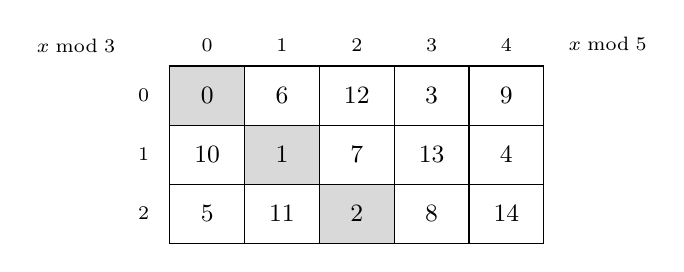
\begin{tikzpicture}[x=0.95cm,y=0.75cm,font=\small]
\foreach \x in {0,...,14}{
  \pgfmathtruncatemacro{\r}{mod(\x,3)}
  \pgfmathtruncatemacro{\c}{mod(\x,5)}
  \ifnum\x<3 \filldraw[fill=gray!30] (\c,-\r) rectangle (\c+1,-\r-1); \else \draw (\c,-\r) rectangle (\c+1,-\r-1); \fi
  \node at (\c+0.5,-\r-0.5) {\x};
}
\foreach \c in {0,...,4}{\node[font=\scriptsize] at (\c+0.5,0.35) {\c};}
\foreach \r in {0,1,2}{\node[font=\scriptsize] at (-0.35,-\r-0.5) {\r};}
\node[anchor=south west,font=\scriptsize] at (5.2,0.1) {$x\bmod5$};
\node[anchor=east,font=\scriptsize] at (-0.6,0.35) {$x\bmod3$};
\end{tikzpicture}
\caption{$\mathbb{Z}/15\mathbb{Z}\to\mathbb{Z}/3\mathbb{Z}\times\mathbb{Z}/5\mathbb{Z}$. $x=0,1,2,\dots$를 차례로 놓으면 행과 열이 함께 하나씩 나아가며(회색은 $0,1,2$) 대각선을 감아 돌고, $15$개 칸을 한 번씩 채운 뒤에야 제자리로 돌아온다.}
\label{fig:crt-grid}
\end{figure}

\cref{fig:crt-grid}은 \cref{thm:crt}를 $m_1=3$, $m_2=5$에서 그린 것이다. 칸 $(x\bmod3,x\bmod5)$에 $x$를 적으면 모든 칸에 정확히 한 수가 들어간다. 행 $2$, 열 $1$의 칸에서 Garner의 방법을 따라가 보자. $v_1=2$이고 $v_2=(1-2)\cdot3^{-1}\bmod5=(-1)\cdot2\bmod5=3$이므로 $x=2+3\cdot3=11$이다. \cref{alg:crt}는 바깥 루프의 $j$번째에서 안쪽 루프를 $j-1$번 도므로 법 연산이 모두 $k(k-1)/2$번이고 역원 표가 $k(k-1)/2$개 필요하다. \code{figures/02/crt.py}는 서로소인 법 몇 묶음에서 무작위 잔여로 \cref{alg:crt}를 돌려 모든 합동을 만족하는지 확인한다.

\begin{algorithm}[htbp]
\begin{algorithmic}[1]
\Require 쌍마다 서로소인 $m_1,\dots,m_k$, 잔여 $a_j\in[0,m_j)$
\Ensure 혼합 기수 자리 $v_1,\dots,v_k$: $x=\sum_jv_j\prod_{i<j}m_i$가 모든 합동을 만족
\For{$j=1,\dots,k$}
  \State $v\gets a_j$
  \For{$i=1,\dots,j-1$} \Comment{지금까지의 $x$를 법 $m_j$로 빼고 $m_i$로 나눈다}
    \State $v\gets\bigl((v-v_i)\bmod m_j\bigr)\cdot(m_i^{-1}\bmod m_j)\bmod m_j$
  \EndFor
  \State $v_j\gets v$
\EndFor
\State \Return $(v_1,\dots,v_k)$
\end{algorithmic}
\caption{Garner의 중국인의 나머지 재구성}
\label{alg:crt}
\end{algorithm}

\cref{alg:crt}의 안쪽 루프는 $v=(a_j-v_1-v_2m_1-\cdots)/(m_1\cdots m_{j-1})\bmod m_j$를 한 자리씩 계산한다. $i$번째 단계가 끝나면 $v\equiv(a_j-\sum_{l\le i}v_l\prod_{l'<l}m_{l'})/(m_1\cdots m_i)\pmod{m_j}$이고 이 식을 $i$에 대한 귀납으로 확인하면 정확성이 나온다. 역원 $m_i^{-1}\bmod m_j$는 법들이 고정이면 미리 한 번 계산해 둔다. 법들이 $2^{32}$보다 작으면 곱 $(v-v_i)\cdot m_i^{-1}$이 $64$비트에 담기므로 기계 정수만으로 충분하고 더 크면 다음 절의 $128$비트 곱이 필요하다.

\subsection{Checksums Modulo a Prime: Adler-32}

나머지 산술이 실제 파일 형식에 쓰이는 예를 보자. stardust의 \code{plot}이 그림을 PNG로 저장할 때 픽셀 데이터는 zlib 형식으로 압축되고 그 끝에 원본 데이터의 Adler-32 체크섬이 붙는다(\code{src/stardust/plot/\_png.py}, RFC 1950\cite{rfc1950}). 바이트 $d_1,\dots,d_n$에 대해 $p=65521$로 두고
\[
A=1+\sum_{i=1}^nd_i\bmod p,\qquad B=\sum_{j=1}^n\Bigl(1+\sum_{i=1}^jd_i\Bigr)\bmod p=n+\sum_{i=1}^n(n-i+1)\,d_i\bmod p
\]
를 계산해 $32$비트 값 $2^{16}B+A$를 만든다. $A$는 바이트의 합이고 $B$는 그 누적합들의 합이다. $p=65521$은 $2^{16}$보다 작은 가장 큰 소수이다(직접 확인했다).

\begin{proposition}
\label{prop:adler-detect}
바이트 하나를 다른 값으로 바꾸면 Adler-32가 반드시 바뀐다. 또한 서로 다른 두 자리 $i<j$의 바이트를 맞바꾸면, $d_i\neq d_j$이고 $j-i<p$인 한 $B$가 반드시 바뀐다.
\end{proposition}

\begin{proof}
$d_i$를 $d_i+\delta$로 바꾸면($0<|\delta|\le255$) $A$는 $\delta\bmod p$만큼 바뀌는데 $|\delta|<p$이므로 $0$이 아니다. 맞바꾸기는 $A$를 바꾸지 않고 $B$를 $(n-i+1)(d_j-d_i)+(n-j+1)(d_i-d_j)=(j-i)(d_j-d_i)$만큼 바꾼다. $p$가 소수이고 $0<j-i<p$, $0<|d_j-d_i|<p$이므로 \cref{thm:unit}에서 두 수 모두 법 $p$의 가역원이고 그 곱도 가역원이어서 $0$이 아니다.
\end{proof}

순진한 구현은 바이트마다 나머지 연산을 두 번 한다. 그런데 \cref{sec:congruence}의 첫 소절에서 본 대로 나머지는 언제 줄여도 되므로 $32$비트 누산기가 넘치지 않는 한 줄이기를 미룰 수 있다. 얼마나 미룰 수 있는지는 다음 명제가 알려 준다.

\begin{proposition}
\label{prop:adler-nmax}
$A,B<p$에서 시작해 바이트 $k$개를 나머지 없이 더하면 $A\le(p-1)+255k$이고 $B\le(p-1)+k(p-1)+255\,k(k+1)/2$이다. 이 한계가 $2^{32}-1$ 이하인 가장 큰 $k$는 $5552$이다.
\end{proposition}

\begin{proof}
바이트가 모두 $255$이고 $A$와 $B$가 모두 $p-1$에서 시작하는 최악을 생각하면 된다. $t$번째 바이트 뒤 $A_t\le(p-1)+255t$이고 $B$는 그 $A_t$들을 더하므로 $B_k\le(p-1)+\sum_{t=1}^k\bigl((p-1)+255t\bigr)=(p-1)+k(p-1)+255\,k(k+1)/2$이다. $k=5552$에서 이 값은 $4\,294\,690\,200<2^{32}=4\,294\,967\,296$이고 $k=5553$에서는 $4\,296\,171\,735$로 넘는다.
\end{proof}

zlib의 상수 \code{NMAX}가 바로 이 $5552$이다. \cref{alg:adler}는 $5552$바이트마다 한 번만 나머지를 구하므로 나눗셈이 바이트당 $2/5552$번으로 줄고, 안쪽 루프는 덧셈 두 번뿐이다. SIMD 구현은 바이트 $16$개를 한 번에 처리하면서 $B$에 $16A+16d_1+15d_2+\cdots+1\cdot d_{16}$을 더한다. 바이트 $16$개 뒤의 $B$ 증가분 $\sum_{t=1}^{16}A_t$를 펼친 것이어서 결과는 같다.

\begin{algorithm}[htbp]
\begin{algorithmic}[1]
\Require 바이트 $d_1,\dots,d_n$, 이전 값 $(A,B)$ (처음이면 $(1,0)$)
\Ensure 이어 붙인 데이터의 $(A,B)$
\State $i\gets1$
\While{$i\le n$}
  \State $k\gets\min(5552,\,n-i+1)$ \Comment{\cref{prop:adler-nmax}: $32$비트에서 넘치지 않는다}
  \For{$t=0,\dots,k-1$} $A\gets A+d_{i+t}$, $B\gets B+A$
  \EndFor
  \State $A\gets A\bmod p$, $B\gets B\bmod p$, $i\gets i+k$
\EndWhile
\State \Return $(A,B)$
\end{algorithmic}
\caption{Adler-32 ($p=65521$, 나머지를 미룬 형태)}
\label{alg:adler}
\end{algorithm}

Adler-32에는 이어 붙이기에 대한 닫힌 공식도 있다. 데이터 $X$와 $Y$의 값을 $(A_X,B_X)$, $(A_Y,B_Y)$라 하고 $Y$의 길이를 $n_Y$라 하면
\[
A_{XY}\equiv A_X+A_Y-1,\qquad B_{XY}\equiv B_X+B_Y+n_Y(A_X-1)\pmod p
\]
이다. $Y$를 처리할 때 $A$가 $1$이 아니라 $A_X$에서 출발하므로 $A$에는 $A_X-1$이 더해지고 $B$에 더해지는 $n_Y$개의 누적합마다 같은 $A_X-1$이 끼기 때문이다. 이 공식이 있으면 데이터를 조각으로 나누어 체크섬을 병렬로 구한 뒤 합칠 수 있다. stardust의 PNG 쓰기는 큰 그림의 압축을 $256$KB 조각으로 나누어 스레드에 맡기지만 Adler-32는 전체 데이터에 대해 한 번 계산한다(\code{zlib.adler32}). 조각마다 구해 이 공식으로 합쳐도 같은 값이 나온다. \code{figures/02/crc\_adler.py}는 \cref{alg:adler}와 결합 공식을 무작위 데이터와 최악의 데이터(모든 바이트가 $255$)에서 zlib과 견주어 확인한다.


\section{Machine Integers}
\label{sec:machine-int}

\subsection{Overflow and Arithmetic Modulo $2^{64}$}

64비트 레지스터는 $[0\,..\,2^{64}-1]$의 정수를 담는다. 두 수를 더하거나 곱한 참값이 이 범위를 넘으면 하드웨어는 넘친 위쪽 비트를 버리고 아래 64비트만 남기는데 남은 값은 정확히 참값을 $2^{64}$로 나눈 나머지이다. 그러므로 부호 없는 64비트 정수의 덧셈과 곱셈은 $\mathbb{Z}/2^{64}\mathbb{Z}$의 연산이며 앞 절에서 본 대로 환의 모든 법칙을 따른다. 특히 덧셈은 결합적이고 교환적이므로 정수의 합은 더하는 순서나 나누어 더하는 방식과 상관없이 같은 비트를 준다. 그래서 정수의 합은 부동소수점 수의 합과 달리 병렬로 계산해도 결과가 하나로 정해진다(17장).

같은 비트 패턴을 다르게 읽으면 부호 있는 정수가 된다. \term{2의 보수}{two's complement} 표현에서는 동치류 $[v]\in\mathbb{Z}/2^{64}\mathbb{Z}$의 대표를 $[0\,..\,2^{64}-1]$ 대신 $[-2^{63}\,..\,2^{63}-1]$에서 고르므로 음수 $v$는 비트 패턴 $v+2^{64}$로 저장되고 맨 위 비트가 $1$인 패턴이 음수를 나타낸다. 이 표현에서는 덧셈과 곱셈이 같은 동치류의 연산이어서 부호가 있든 없든 하드웨어의 덧셈기와 곱셈기를 그대로 쓸 수 있다. 다만 한 가지 함정이 있다. C와 C++ 표준은 부호 있는 정수의 넘침을 정의되지 않은 동작으로 두어서\cite{iso14882-2020} 컴파일러가 ``넘침은 일어나지 않는다''고 가정하고 코드를 변형할 수 있다\cite{lattner2011ub}. 예를 들어 \code{x + 1 > x}는 늘 참으로 접히고, 루프 변수가 넘치지 않는다고 가정해 루프 횟수를 미리 계산한다.

stardust의 정수 연산은 $2^{64}$로 감기는 동작을 약속하므로 부호 있는 정수를 부호 없는 정수로 바꾸어 계산한 뒤 되돌린다(\code{scalar\_ops.hpp}의 \code{wrap\_add}, \code{wrap\_sub}, \code{wrap\_mul}). 부호 있는 정수를 부호 없는 정수로 바꾸는 변환은 표준이 ``$2^{64}$로 나눈 나머지''로 정의하고 그 반대 방향도 C++20부터는 같은 규칙으로 정의되었다. 그래서 이 왕복은 정의된 동작만으로 $\mathbb{Z}/2^{64}\mathbb{Z}$의 연산을 하고, 기계어로는 평범한 \code{ADD}, \code{SUB}, \code{MUL} 한 명령이 된다. \code{negative}는 $0-a$를, \code{abs}는 음수일 때 $0-a$를 감김 뺄셈으로 계산하므로 $-\mathrm{INT\_MIN}=|\mathrm{INT\_MIN}|=\mathrm{INT\_MIN}$이다. $2^{63}$이 $\mathrm{INT\_MIN}$과 같은 동치류에 속하기 때문이다. \code{square}는 감김 곱 $a\cdot a$이고 \code{bitwise\_invert}의 $\lnot a$는 2의 보수에서 $-1-a$이다(\cref{prop:sign-fold}의 증명에서 쓴 사실). \code{sign}은 분기 없이
\[
\operatorname{sign}(a)=(a\gg63)\lor\bigl((0-a)\ggg63\bigr)
\]
로 계산한다. 여기서 $\gg$는 산술 밀기, $\ggg$는 부호 없는 수로 읽은 논리 밀기, $0-a$는 감김 뺄셈이다. $a>0$이면 앞 항이 $0$이고 $0-a=2^{64}-a\ge2^{63}$이어서 뒤 항이 $1$이다. $a=0$이면 둘 다 $0$이다. $\mathrm{INT\_MIN}<a<0$이면 앞 항이 $-1$(모든 비트가 $1$)이어서 결과가 $-1$이고, $a=\mathrm{INT\_MIN}$이면 $0-a=2^{63}$이어서 뒤 항이 $1$이지만 $-1\lor1=-1$이므로 여전히 $-1$이다. 부호 비트를 끌어내리는 비트 연산 두 개가 비교와 분기 두 번을 대신한다.

\begin{aside}[Ariane 5의 첫 비행]
1996년 6월 4일, 유럽우주국의 Ariane 5 로켓은 첫 비행에서 발사 약 40초 만에 궤도를 벗어나 자폭했다. 조사 위원회는 관성 기준 장치의 소프트웨어가 수평 방향 속도와 관련된 64비트 부동소수점 값을 16비트 부호 있는 정수로 바꾸다가 값이 16비트 정수의 범위를 넘어 예외가 났다는 것을 밝혔다\cite{lions1996ariane}. 이 코드는 Ariane 4에서 가져온 것이었는데 Ariane 4의 비행 궤적에서는 그 값이 결코 범위를 넘지 않았기 때문에 넘침에 대한 보호가 빠져 있었다. 그 값의 범위는 계산으로 확인되지 않은 채 가정으로만 남아 있다가 로켓이 바뀌자 깨졌다.
\end{aside}

\subsection{Signed Order and Overflow Detection}

1장의 \cref{alg:float-key}는 양수의 부호 비트를 세워 정렬 키를 만들었다. 정수에 대해 같은 일을 하는 변환이 다음 명제이다.

\begin{proposition}
\label{prop:signflip}
부호 있는 64비트 정수 $v\in[-2^{63}\,..\,2^{63}-1]$의 2의 보수 비트 패턴을 $u=v\bmod2^{64}$라 하자. 맨 위 비트를 뒤집은 $u\oplus2^{63}$을 부호 없는 정수로 읽은 값은 $v+2^{63}$이다. 따라서 부호 있는 정수의 대소는 맨 위 비트를 뒤집은 패턴의 부호 없는 대소와 같다.
\end{proposition}

\begin{proof}
$v\ge0$이면 $u=v<2^{63}$이므로 맨 위 비트가 $0$이고 뒤집으면 $u+2^{63}=v+2^{63}$이다. $v<0$이면 $u=v+2^{64}\ge2^{63}$이므로 맨 위 비트가 $1$이고 뒤집으면 $u-2^{63}=v+2^{63}$이다. 어느 경우든 결과는 $v+2^{63}$이고 이 값은 $v$에 대해 증가한다.
\end{proof}

stardust의 정렬은 int64 값을 기수 정렬할 때 바로 이 변환으로 키를 만들며, 1장의 \cref{prop:float-key}는 부동소수점 수에 대해 같은 생각을 한 걸음 더 밀고 나간다.

감김을 약속하지 않고 넘침을 잡아내야 하는 곳도 있다. 정확한 정수 결과를 내야 하는 통계량의 누산이 그런 예이다. 덧셈의 넘침은 결과의 부호로 판정한다.

\begin{proposition}
\label{prop:add-overflow}
부호 있는 64비트 정수 $a,b$와 감김 합 $r=(a+b)\bmod2^{64}$(2의 보수로 읽음)에 대해 참값 $a+b$가 범위 $[-2^{63},2^{63})$을 벗어날 필요충분조건은 $a$와 $b$의 부호가 같고 $r$의 부호가 그와 다른 것이다. 비트 연산으로는 $(a\oplus r)\land(b\oplus r)$의 맨 위 비트가 $1$인 것과 같다.
\end{proposition}

\begin{proof}
부호가 다르면 $|a+b|\le\max(|a|,|b|)$여서 넘치지 않고 이때 $r=a+b$의 부호는 둘 중 하나와 같다. 부호가 같고 둘 다 음이 아니면 참값은 $[0,2^{64}-2]$에 있고 $2^{63}$ 이상일 때만 넘치며 그때 $r=a+b-2^{64}<0$이다. 둘 다 음수이면 참값은 $[-2^{64},-2]$에 있고 $-2^{63}$ 미만일 때만 넘치며 그때 $r=a+b+2^{64}\ge0$이다. 비트 식은 ``$r$의 부호가 $a$와도 다르고 $b$와도 다르다''를 적은 것이다.
\end{proof}

stardust의 비모수 검정은 통계량의 정확한 값을 \code{\_\_int128}(GCC와 Clang이 제공하는 $128$비트 정수)로 누산해 이 걱정을 피한다(\code{csrc/htest/rank.cpp}의 \code{T3}, \code{gof2.cpp}의 \code{U4}). 동점 보정항 $\sum(t^3-t)$처럼 표본 크기의 세제곱으로 자라는 값도 $128$비트에는 넉넉히 담긴다.

곱셈의 넘침은 덧셈처럼 부호만 보고 판정할 수 없다. 대신 곱의 위쪽 절반을 본다.

\begin{proposition}
\label{prop:mul-overflow}
부호 있는 64비트 정수 $a,b$의 곱을 $128$비트 2의 보수로 적어 위쪽 $64$비트를 $h$, 아래쪽 $64$비트를 $l$이라 하자. 참값 $ab$가 $[-2^{63},2^{63})$에 들 필요충분조건은 $h$가 $l$의 맨 위 비트를 $64$번 늘인 값, 곧 $h=l\gg63$(산술 밀기)인 것이다.
\end{proposition}

\begin{proof}
$|ab|\le2^{126}$이므로 $ab$는 $128$비트 2의 보수로 정확히 나타난다. $128$비트 패턴이 $[-2^{63},2^{63})$의 수를 나타낼 필요충분조건은 위 $65$비트가 모두 같은 것, 곧 부호 비트가 $64$번째 자리부터 확장된 꼴인 것이다. 이것이 $h$의 모든 비트가 $l$의 맨 위 비트와 같다는 조건이다.
\end{proof}

AArch64에서는 $l$을 \code{MUL}이, $h$를 \code{SMULH}가 주므로 판정은 명령 세 개이다. Clang은 \code{\_\_builtin\_mul\_overflow}를 \code{MUL}, \code{SMULH}, 그리고 $h$와 $l\gg63$을 견주는 \code{CMP} 하나로 옮긴다(이 책의 측정 기계에서 어셈블리를 확인했다). stardust는 이 내장 함수를 shape의 원소 수나 결과 배열의 크기를 계산하는 곳에서 쓴다(\code{csrc/array/ops/shape.cpp}, \code{csrc/linalg/batch.cpp} 등). 축 길이의 곱이 넘치면 감긴 작은 값으로 메모리를 잡는 대신 \code{ValueError}(``array is too big'')를 낸다. 원소 연산에서는 감김을 약속하지만 배열의 크기는 감기면 메모리 안전이 깨지므로 두 곳의 정책이 다르다.

\subsection{Shifts}

비트 밀기는 $2$의 거듭제곱을 곱하거나 나누는 연산이다.

\begin{proposition}
\label{prop:shift-floor}
$0\le s\le63$이라 하자. 부호 있는 64비트 정수 $a$에 대해 산술 오른쪽 밀기 $a\gg s$(빈 자리를 부호 비트로 채움)는 $\lfloor a/2^s\rfloor$이고, 왼쪽 밀기 $a\ll s$는 $2^sa\bmod2^{64}$이다.
\end{proposition}

\begin{proof}
왼쪽 밀기는 비트 $b_i$를 $b_{i+s}$로 옮기고 $64$번 이상의 자리를 버리므로 $2^sa$를 $2^{64}$로 나눈 나머지이다. 오른쪽 밀기를 보자. $a\ge0$이면 비트 패턴이 $a$의 이진 전개이고 아래 $s$비트를 버리는 것은 $\lfloor a/2^s\rfloor$이다. $a<0$이면 패턴 $u=a+2^{64}$의 아래 $s$비트를 버리고 위에 $1$을 $s$개 채우므로 결과 패턴은 $\lfloor u/2^s\rfloor+2^{64}-2^{64-s}$이고 이 패턴을 2의 보수로 읽으면 $\lfloor u/2^s\rfloor-2^{64-s}=\lfloor(u-2^{64})/2^s\rfloor=\lfloor a/2^s\rfloor$이다.
\end{proof}

\cref{prop:shift-floor}에서 산술 오른쪽 밀기는 F-나눗셈이다. $-7\gg1=-4$이고 C의 \code{-7 / 2}는 $-3$이다. 그래서 컴파일러는 부호 있는 정수를 $2$의 거듭제곱으로 나누는 \code{a / 2} 같은 T-나눗셈을 밀기 하나로 바꾸지 못하고 음수일 때 $2^s-1$을 더하는 보정을 붙인다. 반대로 \cref{alg:magic}의 첫 줄처럼 바닥 나눗셈은 밀기 하나로 끝난다.

밀기 셈의 범위 밖에서는 언어와 하드웨어가 갈라진다. C++에서 셈이 음수이거나 $64$ 이상이면 정의되지 않은 동작이다. AArch64의 \code{LSLV}와 \code{ASRV}는 셈을 $64$로 나눈 나머지만 쓰므로 \code{1 << 64}를 하드웨어에 맡기면 $1$이 나온다(x86도 같다). stardust는 모든 비트가 밀려 나가는 답을 택했다. 수학적으로는 이쪽이 자연스럽다. \cref{alg:shifts}는 셈을 부호 없는 정수로 읽어 음수 셈을 큰 양수로 보내고 셈이 $64$ 이상이면 왼쪽 밀기는 $0$, 오른쪽 밀기는 부호에 따라 $0$이나 $-1$을 준다. $-1$은 \cref{prop:shift-floor}을 셈이 무한히 커지는 극한으로 늘린 값, 곧 음수를 $2^s$로 나눈 바닥의 극한이다.

\begin{algorithm}[htbp]
\begin{algorithmic}[1]
\Require 부호 있는 64비트 정수 $a$와 셈 $b$
\Function{LeftShift}{$a,b$}
  \State \textbf{if} $b$를 부호 없는 수로 읽어 $64$ 이상 \textbf{then} \Return $0$ \Comment{음수 셈도 여기로}
  \State \Return $a$를 부호 없는 수로 바꿔 $b$비트 왼쪽으로 민 값 \Comment{부호 있는 넘침을 피한다}
\EndFunction
\Function{RightShift}{$a,b$}
  \State \textbf{if} $b$를 부호 없는 수로 읽어 $64$ 이상 \textbf{then} \Return ($a<0$ ? $-1$ : $0$)
  \State \Return $a\gg b$ (산술 밀기) \Comment{$\lfloor a/2^b\rfloor$}
\EndFunction
\end{algorithmic}
\caption{밀기 셈의 경계 처리 (stardust \code{bitwise\_left\_shift}, \code{bitwise\_right\_shift})}
\label{alg:shifts}
\end{algorithm}

\cref{tab:int-edges}에서는 이 장의 정수 규칙이 드러나는 경계값마다 stardust의 규칙(\code{docs/design/array.md} §2.3과 \code{scalar\_ops.hpp})과 numpy 2.5.5의 실제 결과를 견준다(\code{figures/02/numpy\_edges.py}). 값이 다른 곳은 둘이다. numpy는 $a\mathbin{\%}0$을 $0$으로 주어 $a=(a\mathbin{/\!/}b)\,b+a\mathbin{\%}b$를 깨고 정수의 음의 지수를 오류로 거부한다. 그 밖에 numpy는 몇몇 경우에 경고를 내지만 stardust는 원소 연산에서 경고를 내지 않는다.

\begin{table}[htbp]
\begin{sdtable}{colspec={lll}, row{1}={font=\small\bfseries}}
\toprule
식 (int64) & stardust & numpy 2.5.5 \\
\midrule
\code{INT\_MIN // -1} & $\mathrm{INT\_MIN}$ & $\mathrm{INT\_MIN}$ (넘침 경고) \\
\code{7 // 0} & $0$ & $0$ (0으로 나눔 경고) \\
\code{7 \% 0} & $7$ & $0$ (0으로 나눔 경고) \\
\code{abs(INT\_MIN)}, \code{-INT\_MIN} & $\mathrm{INT\_MIN}$ & $\mathrm{INT\_MIN}$ \\
\code{INT\_MAX + 1} & $\mathrm{INT\_MIN}$ & $\mathrm{INT\_MIN}$ \\
\code{1 << 64}, \code{1 << -1} & $0$ & $0$ \\
\code{-8 >> 64}, \code{-8 >> -1} & $-1$ & $-1$ \\
\code{2 ** -1} & $0$ & \code{ValueError} \\
\code{3 ** 41} & $-420491770248316829$ & $-420491770248316829$ \\
\bottomrule
\end{sdtable}
\caption{정수 경계값에서 stardust의 규칙과 numpy의 결과.}
\label{tab:int-edges}
\end{table}

\subsection{Powers by Repeated Squaring}

정수 거듭제곱 $a^e$는 $e$를 이진법으로 적어 $a,a^2,a^4,\dots$을 차례로 제곱하며 필요한 것만 곱한다. 감김 산술에서 이렇게 해도 되는 이유는 $a\mapsto[a]$가 환 준동형이어서 $[a^e]=[a]^e$이기 때문이다. 곧 중간 결과를 $2^{64}$로 줄여 가며 계산한 값은 참값 $a^e$를 $2^{64}$로 나눈 나머지와 같다. \cref{tab:int-edges}의 $3^{41}$은 Python의 큰 정수로 계산해 줄인 값과 같다.

\begin{algorithm}[htbp]
\begin{algorithmic}[1]
\Require 부호 있는 64비트 정수 $a$, $e$
\Ensure $a^e$를 $2^{64}$로 감은 값 ($e<0$이면 정수 결과의 규칙)
\If{$e<0$} \Comment{역수가 정수인 밑은 $\pm1$뿐}
  \State \Return ($a=1$ ? $1$ : $a=-1$ ? $(-1)^e$ : $0$)
\EndIf
\State $r\gets1$
\While{$e\neq0$} \Comment{불변식: $r\cdot a^e$가 처음의 $a^e$와 같다 (법 $2^{64}$)}
  \State \textbf{if} $e$가 홀수 \textbf{then} $r\gets r\cdot a$ (감김)
  \State $e\gets e\gg1$
  \State \textbf{if} $e\neq0$ \textbf{then} $a\gets a\cdot a$ (감김) \Comment{마지막 제곱은 쓰지 않으므로 건너뛴다}
\EndWhile
\State \Return $r$
\end{algorithmic}
\caption{제곱을 거듭하는 정수 거듭제곱 (stardust \code{pow}의 정수 커널)}
\label{alg:int-pow}
\end{algorithm}

\cref{alg:int-pow}의 불변식은 $e$가 홀수이면 $r\cdot a^e=(ra)\cdot(a^2)^{(e-1)/2}$이고 짝수이면 $r\cdot(a^2)^{e/2}$라는 데서 유지된다. 루프는 $e$의 비트 수인 $\lfloor\log_2e\rfloor+1$번 돌고 곱셈은 $\lfloor\log_2e\rfloor+\operatorname{popcount}(e)$번 한다. 8행의 조건은 마지막 반복에서 쓰이지 않을 제곱을 건너뛰는 것이다. 감김 산술에서는 그 제곱이 결과를 바꾸지 않으므로 순전히 비용을 아끼는 장치이다. 음의 지수는 $a^{-1}$이 정수인 $a=\pm1$만 정수 결과를 가진다. stardust는 나머지 경우를 $0$으로 정했다. $0^{-n}$도 $0$인데 이것은 $0$으로 나누기의 규칙($a\mathbin{/\!/}0=0$)과 맞춘 것이다.

\subsection{Inverses Modulo $2^{64}$}

\cref{thm:unit}에서 홀수 $a$는 $\mathbb{Z}/2^{64}\mathbb{Z}$의 가역원이다. 역원은 \cref{alg:ext-euclid}로도 구할 수 있지만 $2$의 거듭제곱을 법으로 할 때는 곱셈 몇 번으로 끝나는 훨씬 빠른 방법이 있다. 실수에서 $1/a$를 구하는 Newton 방법을 그대로 정수에 옮기면 된다\cite{warren2012hackers}.

\begin{proposition}
\label{prop:hensel}
홀수 $a$와 정수 $x$가 $ax\equiv1\pmod{2^k}$를 만족하면 $x'=x(2-ax)$는 $ax'\equiv1\pmod{2^{2k}}$를 만족한다. 또한 모든 홀수 $a$에 대해 $a\cdot a\equiv1\pmod8$이고 $a\cdot\bigl((3a)\oplus2\bigr)\equiv1\pmod{32}$이다.
\end{proposition}

\begin{proof}
$ax=1+e$이고 $2^k$가 $e$를 나눈다고 하자. 그러면 $ax'=ax(2-ax)=(1+e)(1-e)=1-e^2$이고, $2^{2k}$가 $e^2$을 나누므로 $ax'\equiv1\pmod{2^{2k}}$이다. 둘째 주장은 $a=2j+1$로 쓰면 $a^2=4j(j+1)+1$이고 $j(j+1)$이 짝수라는 데서 나온다. 셋째 주장은 $(3a)\oplus2$의 아래 $5$비트가 $a$의 아래 $5$비트로 정해지므로 $a\bmod32$의 홀수 $16$가지를 모두 확인하면 된다(\code{figures/02/newton\_inverse.py}가 확인한다).
\end{proof}

\cref{prop:hensel}에 따라 $x_0=a$에서 시작하면 $x_0$은 아래 $3$비트가 맞고 한 번 갱신할 때마다 맞는 비트의 수가 두 배가 되어 $6,12,24,48$을 거쳐 다섯 번 만에 $96\ge64$비트, 곧 정확한 역원에 이른다. $x_0=(3a)\oplus2$에서 시작하면 $5,10,20,40,80$이어서 네 번으로 충분하다. \cref{tab:newton-bits}는 무작위 홀수 $10^5$개에서 잰 맞는 비트 수의 최솟값으로 이 예측과 정확히 맞는다. 이 방법은 \term{Hensel 올림}{Hensel lifting}의 가장 간단한 예이며 법을 $2^k$에서 $2^{2k}$로 키워 가며 해를 끌어올린다고 볼 수 있다.

\begin{algorithm}[htbp]
\begin{algorithmic}[1]
\Require 홀수 $a$ (부호 없는 64비트)
\Ensure $a\,x\equiv1\pmod{2^{64}}$
\State $x\gets(3a)\oplus2$ \Comment{아래 $5$비트가 맞다}
\For{$4$번} $x\gets x\,(2-ax)$ (감김) \Comment{맞는 비트: $10,20,40,80$}
\EndFor
\State \Return $x$
\end{algorithmic}
\caption{$2^{64}$를 법으로 한 역원 (Newton 반복)}
\label{alg:inverse-2k}
\end{algorithm}

\begin{table}[htbp]
\begin{sdtable}{colspec={lcccccc}, row{1}={font=\small\bfseries}}
\toprule
출발점 & $x_0$ & $x_1$ & $x_2$ & $x_3$ & $x_4$ & $x_5$ \\
\midrule
$x_0=a$ & $3$ & $6$ & $12$ & $24$ & $48$ & $64$ \\
$x_0=(3a)\oplus2$ & $5$ & $10$ & $20$ & $40$ & $64$ & $64$ \\
\bottomrule
\end{sdtable}
\caption{Newton 반복의 맞는 아래 비트 수(무작위 홀수 $10^5$개의 최솟값, \code{figures/02/newton\_inverse.py}).}
\label{tab:newton-bits}
\end{table}

역원의 쓸모는 둘이다. 첫째, $d$가 홀수이고 $a$가 $d$의 배수임을 미리 알면 $a/d=a\cdot d^{-1}\bmod2^{64}$이다. $a=qd$이면 $ad^{-1}\equiv q$이고 $q$가 범위 안에 있으므로 나머지가 곧 몫이다. 나누어떨어지는 나눗셈을 곱셈 하나로 바꾸는 이 방법은 \cref{prop:score-lattice}처럼 $g$로 나누어떨어짐을 아는 계산에서 쓸 수 있다. 둘째, 곱셈이 전단사라는 것을 구체적으로 보여 준다. Philox의 곱수 $\code{0xD2E7470EE14C6C93}$과 $\code{0xCA5A826395121157}$의 역원은 각각 $\code{0x6C6D4A4B2DB9919B}$, $\code{0x17DF77E820BB6A67}$이고 이것으로 \cref{sec:bijection}에서 Philox의 한 라운드를 거꾸로 돌린다.

홀수의 쓸모는 덧셈에도 있다. \cref{prop:cyclic}을 $M=2^{64}$에 쓰면 홀수 $w$를 거듭 더하는 \term{Weyl 수열}{Weyl sequence} $k,k+w,k+2w,\dots$은 $2^{64}$개의 값을 모두 한 번씩 지난 뒤에야 처음으로 돌아온다. 특히 $i\ne j$이고 $|i-j|<2^{64}$이면 $k+iw\ne k+jw$이다. $(i-j)w\equiv0$이면 $w$가 가역이므로 $i-j\equiv0$이기 때문이다. Philox는 라운드 사이마다 열쇠에 $\code{0x9E3779B97F4A7C15}=\lfloor2^{64}(\varphi-1)\rfloor$와 $\code{0xBB67AE8584CAA73B}=\lfloor2^{64}(\sqrt3-1)\rfloor$를 더한다(\code{csrc/random/philox.hpp}, 두 값 모두 직접 계산해 확인했다). 라운드는 열 번뿐이므로 주기가 최대라는 것 자체는 쓰이지 않는다. 쓰이는 것은 두 상수가 홀수여서 열 라운드의 열쇠가 서로 다르다는 사실이고, 무리수의 소수 부분을 고른 것은 열쇠의 비트가 규칙적이지 않게 하려는 것이다.

\subsection{The High Half of a Product}

두 64비트 정수의 곱은 최대 128비트이다. 하드웨어에는 곱의 아래 64비트와 위 64비트를 따로 얻는 명령이 있고(AArch64에서는 \code{MUL}과 \code{UMULH}) 위쪽 절반은 곱을 $2^{64}$로 나눈 몫이다. C++ 표준에는 $128$비트 정수가 없지만 GCC와 Clang의 \code{unsigned \_\_int128}로 곱하고 $64$비트 밀면 컴파일러가 \code{UMULH} 한 명령으로 바꾼다. stardust의 Philox도 이렇게 쓴다(\code{mulhilo}). 이 확장이 없는 컴파일러에서는 $32$비트 조각으로 직접 계산해야 한다(\cref{alg:mulhi}).

\begin{algorithm}[htbp]
\begin{algorithmic}[1]
\Require 부호 없는 64비트 정수 $a=2^{32}a_1+a_0$, $b=2^{32}b_1+b_0$
\Ensure $\lfloor ab/2^{64}\rfloor$
\State $p_{00}\gets a_0b_0$, $p_{01}\gets a_0b_1$, $p_{10}\gets a_1b_0$, $p_{11}\gets a_1b_1$ \Comment{각각 $<2^{64}$}
\State $c\gets(p_{00}\gg32)+(p_{01}\bmod2^{32})+(p_{10}\bmod2^{32})$ \Comment{$<3\cdot2^{32}$: 넘치지 않는다}
\State \Return $p_{11}+(p_{01}\gg32)+(p_{10}\gg32)+(c\gg32)$
\end{algorithmic}
\caption{$32$비트 조각으로 곱의 위쪽 절반}
\label{alg:mulhi}
\end{algorithm}

\cref{alg:mulhi}의 정확성은 $ab=2^{64}p_{11}+2^{32}(p_{01}+p_{10})+p_{00}$을 $2^{32}$ 단위의 자리로 다시 묶는 데서 나온다. 2행의 $c$는 $2^{32}$ 자리에 모이는 것들의 합이고 그 위쪽이 $2^{64}$ 자리로 올라간다. 각 조각이 $2^{32}$ 미만이므로 $c<3\cdot2^{32}$이어서 $64$비트에 담기고 3행의 합은 참값 $\lfloor ab/2^{64}\rfloor<2^{64}$와 같으므로 역시 넘치지 않는다.

\subsection{Uniform Integers in a Range}

곱의 위쪽 절반이 쓰이는 대표적인 곳이 균등한 64비트 난수 $w$에서 $[0\,..\,r-1]$의 균등한 정수를 얻는 문제이다. 가장 손쉬운 방법은 $w\bmod r$이지만 두 가지 문제가 있다. 정수 나눗셈은 곱셈보다 느리고, $2^{64}$이 $r$의 배수가 아니면 $2^{64}\bmod r$보다 작은 값들이 한 번씩 더 나와 분포가 치우친다. Lemire의 방법은 나눗셈 대신 곱의 위쪽 절반 $\lfloor wr/2^{64}\rfloor$를 쓰고, 치우침을 없애기 위해 곱의 아래쪽 절반이 작은 경우만 골라 버린다\cite{lemire2019interval}.

\begin{theorem}
\label{thm:lemire}
$1\le r\le2^{64}$이고 $t=2^{64}\bmod r$이라 하자. $w\in[0\,..\,2^{64}-1]$에 대해 $wr=j\,2^{64}+l$, $0\le l<2^{64}$로 쓸 때, $l\ge t$인 $w$만 받아들이고 $j$를 출력하면 각 $j\in[0\,..\,r-1]$은 정확히 $\lfloor2^{64}/r\rfloor$개의 $w$에서 나온다. 따라서 $w$가 균등하면 받아들인 $w$가 주는 $j$도 균등하다.
\end{theorem}

\begin{proof}
$j$를 고정하자. $\lfloor wr/2^{64}\rfloor=j$인 $w$는 $j\,2^{64}\le wr<(j+1)2^{64}$인 정수들이고 그 아래쪽 절반 $l=wr-j\,2^{64}$은 $w$가 $1$ 늘 때마다 $r$씩 느는 등차수열을 이루며 $[0\,..\,2^{64}-1]$을 지나간다. 또 이 수열의 모든 항은 실제로 정의역 안의 $w$에서 나온다. $w<(j+1)2^{64}/r\le2^{64}$이기 때문이다. 이제 $2^{64}=qr+t$, $q=\lfloor2^{64}/r\rfloor$로 쓰면 받아들이는 구간 $[t,2^{64})$의 길이는 정확히 $qr$이다. 공차가 $r$인 등차수열은 길이가 $qr$인 반열린 구간에 정확히 $q$개의 항이 있으므로 받아들이는 $w$는 $j$에 상관없이 정확히 $q$개이다.
\end{proof}

\cref{tab:lemire}는 단어의 길이를 $64$비트가 아니라 $3$비트로 줄여 $r=3$에 대해 이 과정을 따라간다. $2^3=8=2\cdot3+2$이므로 $t=2$이고 받아들인 여섯 개의 $w$가 $0$, $1$, $2$를 두 번씩 낸다. \code{figures/02/lemire\_bias.py}는 $8$비트와 $12$비트 단어에서 모든 $r$에 대해 \cref{thm:lemire}를 전수로 확인한다.

\begin{table}[htbp]
\begin{sdtable}{colspec={ccccccccc}, row{1}={font=\small\bfseries}}
\toprule
$w$ & 0 & 1 & 2 & 3 & 4 & 5 & 6 & 7 \\
\midrule
$wr$ & 0 & 3 & 6 & 9 & 12 & 15 & 18 & 21 \\
$j=\lfloor wr/8\rfloor$ & 0 & 0 & 0 & 1 & 1 & 1 & 2 & 2 \\
$l=wr\bmod8$ & 0 & 3 & 6 & 1 & 4 & 7 & 2 & 5 \\
$l\ge t$ & 버림 & 받음 & 받음 & 버림 & 받음 & 받음 & 받음 & 받음 \\
\bottomrule
\end{sdtable}
\caption{$3$비트 단어와 $r=3$에서 따라간 Lemire의 방법. $t=8\bmod3=2$이고, 받아들인 $w$는 $j=0,1,2$를 정확히 두 번씩 낸다.}
\label{tab:lemire}
\end{table}

버림의 확률은 $t/2^{64}<r/2^{64}$이다. $r$이 작으면 무시할 만하지만 $r$이 $2^{63}$을 조금 넘으면 $t=2^{64}-r$이 거의 $2^{63}$이어서 절반 가까이 버린다. \cref{fig:lemire}에는 $16$비트 단어로 줄인 같은 상황에서 $r$에 따른 버림 확률을 그렸다. $r$이 $2^{16}/k$를 조금 넘을 때마다 톱니가 솟는다. 같은 그림에서 $w\bmod r$의 치우침이 어디서 큰지도 읽을 수 있다. 나머지 방법에서 $t$개의 값이 $q+1$번, 나머지가 $q$번 나오므로 상대적 치우침은 $1/q$이다.

\begin{figure}[htbp]
\centering
\begin{tikzpicture}
\begin{semilogxaxis}[sdplot,xlabel={$r$},ylabel={버림 확률},xmin=256,xmax=65536,ymin=0,ymax=0.55,log basis x=2,xtick={256,1024,4096,16384,65536}]
\addplot[black,thin,mark=none] table[x=r,y=reject]{figures/02/lemire_bias.dat};
\addlegendentry{$t/2^{16}$}
\addplot[black,dashed,domain=256:65536,samples=60] {x/65536};
\addlegendentry{$r/2^{16}$}
\end{semilogxaxis}
\end{tikzpicture}
\caption{$16$비트 단어에서 Lemire의 방법이 버리는 확률 $t/2^{16}$ ($t=2^{16}\bmod r$, \code{figures/02/lemire\_bias.py}). 점선은 한계 $r/2^{16}$이고, $r$이 $2$의 거듭제곱이면 $t=0$이어서 버리지 않는다. $r<2^8$에서는 확률이 $2^{-8}$ 미만이다.}
\label{fig:lemire}
\end{figure}

$t=2^{64}\bmod r$을 계산하려면 나눗셈이 한 번 필요하지만 $t<r$이므로 먼저 $l<r$인지만 보고 그럴 때에만 $t$를 구하면 대부분의 경우 나눗셈을 아예 하지 않는다. $l<r$일 확률은 $r/2^{64}$이다. 또한 $2^{64}$은 64비트에 담기지 않으므로 $t$를 그대로 적을 수 없는데 부호 없는 산술에서 $0-r$은 $2^{64}-r$이고 $(2^{64}-r)\bmod r=2^{64}\bmod r$이므로 \code{(0 - r) \% r}로 계산하면 된다. \cref{alg:bounded}는 stardust의 \code{bounded}이다(\code{csrc/random/philox.hpp}). 범위를 원소마다 다르게 주는 \code{integers}(범위가 배열인 경우)와 \code{permutation}의 섞기(Fisher–Yates의 각 단계에서 남은 원소 가운데 하나를 고른다)가 이 함수를 쓴다.

\begin{algorithm}[htbp]
\begin{algorithmic}[1]
\Require 원소 $e$의 첫 단어 $w$, 범위 $r$ ($r=0$은 $2^{64}$을 뜻함), 여분 단어의 출처 $\mathrm{extra}_e(0),\mathrm{extra}_e(1),\dots$
\Ensure $[0,r)$의 균등한 정수
\State \textbf{if} $r=0$ \textbf{then} \Return $w$
\State $(h,l)\gets$ $wr$의 위쪽과 아래쪽 절반 \Comment{\code{UMULH}, \code{MUL}}
\If{$l<r$} \Comment{확률 $r/2^{64}$: 이때만 나눗셈}
  \State $t\gets(0-r)\bmod r$ \Comment{$=2^{64}\bmod r$}
  \State $k\gets0$
  \While{$l<t$} \Comment{\cref{thm:lemire}의 버림}
    \State $(h,l)\gets\mathrm{extra}_e(k)\cdot r$의 두 절반, $k\gets k+1$
  \EndWhile
\EndIf
\State \Return $h$
\end{algorithmic}
\caption{범위의 균등한 정수 (stardust \code{bounded})}
\label{alg:bounded}
\end{algorithm}

7행의 여분 단어가 구현에서 가장 신경 쓴 부분이다. stardust의 난수는 계수기 방식이어서 원소 $e$의 첫 단어는 계수기 $(\lfloor e/4\rfloor,0,0,0)$ 블록의 $e\bmod4$번째 단어로 정해져 있다. 버림이 일어날 때 다음 원소의 단어를 빌려 쓰면 그 뒤의 모든 원소가 한 칸씩 밀리고 결과가 스레드 분할에 따라 달라진다. 그래서 원소마다 따로 된 여분 단어의 흐름 $(e,1+\lfloor k/4\rfloor,0,0)$ 블록을 두어 버림이 그 원소 안에서만 끝나게 했다. 두 번째 성분이 $0$인 계수기와 $1$ 이상인 계수기는 결코 만나지 않으므로 같은 단어를 두 번 쓰지 않는다. 계수기 방식과 스레드 결정성은 X권의 난수 생성에서 자세히 다룬다.

범위가 하나뿐인 보통의 \code{integers(low, high)}는 따로 짠 경로를 탄다(\cref{alg:integers}, \code{csrc/random/random.cpp}의 \code{integers}). 범위가 모든 원소에서 같으므로 $t$를 호출마다 한 번만 구해 두고, 원소마다 $l<r$ 검사 없이 $l<t$를 바로 비교한다. $r=2^{63}+1$ 근처에서는 단어의 절반쯤을 버리므로 \cref{alg:bounded}처럼 원소마다 $t$를 구하는 쪽이 오히려 나눗셈을 자주 하게 되기 때문이다.

\begin{algorithm}[htbp]
\begin{algorithmic}[1]
\Require 부호 있는 64비트 정수 $\ell\le h$, \code{endpoint}, 원소 수 $n$, 원소 $i$의 첫 단어 $w_i$
\Ensure $o_i$: $[\ell,h)$ (\code{endpoint}이면 $[\ell,h]$)의 균등한 정수
\State $r\gets(h-\ell)+[\code{endpoint}]$ (부호 없는 감김 산술) \Comment{$r=0$은 $2^{64}$을 뜻한다}
\State $t\gets(r=0)\ ?\ 0:(0-r)\bmod r$ \Comment{호출마다 한 번}
\If{$r=0$} $o_i\gets\ell+w_i$ (감김) \textbf{for all} $i$; \Return
\EndIf
\If{$r\le2^{60}$} \Comment{버림 확률 $<2^{-4}$}
  \For{$i=0,\dots,n-1$} $(j_i,\lambda_i)\gets w_ir$; \textbf{while} $\lambda_i<t$: 여분 단어로 다시; $o_i\gets\ell+j_i$
  \EndFor
\Else \Comment{버림이 잦다: 분기 없이 모은다}
  \For{$i=0,\dots,n-1$}
    \State $(j_i,\lambda_i)\gets w_ir$, $o_i\gets\ell+j_i$, $\mathit{rej}[c]\gets i$, $c\gets c+[\lambda_i<t]$
    \State \textbf{if} $c=B$ \textbf{then} \Call{Finish}{}, $c\gets0$
  \EndFor
  \State \Call{Finish}{} \Comment{모인 원소 넷씩: 여분 단어 블록을 \code{philox4}로 함께 계산해 다시 뽑는다}
\EndIf
\end{algorithmic}
\caption{범위가 하나인 \code{integers} (stardust)}
\label{alg:integers}
\end{algorithm}

\cref{alg:integers}의 1행은 범위의 폭을 부호 없는 산술로 구한다. $\ell\le h$이면 참값 $h-\ell$은 $[0,2^{64})$에 있으므로 정확하고, \code{endpoint}로 $1$을 더한 값이 $2^{64}$이 되면 $0$으로 감기는데 이것이 \cref{alg:bounded}의 ``$r=0$은 전체 범위'' 약속과 맞는다. 결과 $o_i=\ell+j_i$($j_i\in[0,r)$는 곱의 위쪽 절반, $\lambda_i$는 아래쪽 절반)도 감김 덧셈으로 구하지만 참값이 $[\ell,h]$ 안이어서 부호 있는 범위에 들어가므로 감긴 값이 곧 참값이다. 3행의 전체 범위에서는 단어가 곧 답이다. 5--13행이 경로를 둘로 나눈 까닭은 분기 예측이다. $r\le2^{60}$이면 버림이 드물어 6행의 \textbf{while}이 거의 돌지 않는다. $r$이 $2^{63}$을 조금 넘으면 단어의 절반쯤을 버리므로 버림 여부로 분기하면 예측이 절반쯤 빗나간다. 10행은 모든 원소가 후보 값과 자기 번호를 쓰되 버림일 때만 계수 $c$를 늘려서 분기를 없앤다. 버린 원소는 넷씩 묶어 첫 여분 블록(여분 단어 $0$--$3$)을 \code{philox4}로 함께 계산하고(곱셈 사슬 넷을 엇갈려 돌린다), 그래도 버려지면 다음 블록을 하나씩 계산한다. 어느 경로든 원소마다 같은 단어를 같은 순서로 쓰므로 결과는 \cref{alg:bounded}를 원소마다 부른 것과 비트까지 같고 스레드 수와도 무관하다.

같은 파일의 \code{to\_unit}은 $w$에서 $[0,1)$의 실수를 만든다. 위 $53$비트 $w\gg11$에 $2^{-53}$을 곱하는데 $53$비트 정수는 binary64에 정확히 담기고 $2$의 거듭제곱을 곱하는 것도 정확하므로 결과는 $\{0,2^{-53},2\cdot2^{-53},\dots,1-2^{-53}\}$의 값을 각각 확률 $2^{-53}$로 정확히 낸다. 근거는 둘이다. 첫째, binary64의 유효숫자는 $53$비트이므로 $0\le k<2^{53}$인 정수 $k$는 정확히 나타난다. 둘째, $k\ne0$이면 $k\cdot2^{-53}\ge2^{-53}$은 정규 수의 범위에 있으므로 $2^{-53}$을 곱하는 것은 지수만 $53$ 줄이고 유효숫자를 건드리지 않는다. 또 $w$가 균등하면 $k=w\gg11$의 값마다 $w$가 $2^{11}$개씩 대응하므로 $k$도 균등하다. binary64의 구조는 10장에서 자세히 다룬다.


\section{Bijections and Bit Mixing}
\label{sec:bijection}

난수 생성기와 해시 함수는 입력의 비트를 골고루 섞는 함수를 필요로 한다. 이때 섞는 함수가 \textbf{전단사}이면 큰 이점이 있다. 서로 다른 입력이 결코 같은 출력으로 가지 않으므로 예컨대 서로 다른 계수기 값에서 같은 난수 블록이 나오는 일이 원리적으로 불가능하고 서로 다른 정수 키가 섞인 뒤 같은 해시가 되는 일도 없다. 이 절은 전단사의 부품과 그 역함수, 섞임의 정도를 재는 기준, 그리고 stardust의 해시와 난수가 그 부품으로 어떻게 짜였는지를 본다.

\subsection{Bijective Building Blocks}

\begin{proposition}
\label{prop:bijections}
$\mathbb{Z}/2^{64}\mathbb{Z}$ 위에서 다음 함수들은 전단사이다.
\begin{enumerate}
\item 홀수 $a$를 곱하는 $x\mapsto ax$. 역함수는 $x\mapsto a^{-1}x$이다.
\item 상수 $k$를 더하는 $x\mapsto x+k$, 그리고 상수와 비트별 배타적 논리합을 하는 $x\mapsto x\oplus k$.
\item $1\le s\le63$에 대해 오른쪽으로 밀어 배타적 논리합을 하는 $x\mapsto x\oplus(x\gg s)$.
\end{enumerate}
또한 전단사의 합성은 전단사이다.
\end{proposition}

\begin{proof}
(i)과 (ii)는 역함수가 분명하다. (iii)을 보자. $y=x\oplus(x\gg s)$라 하면 $y$의 맨 위 $s$비트는 $x\gg s$의 해당 비트가 $0$이므로 $x$의 맨 위 $s$비트와 같다. 그다음 $s$비트는 $x$의 해당 비트와, 이미 알아낸 맨 위 $s$비트의 배타적 논리합이므로 역시 알아낼 수 있다. 이렇게 위에서부터 $s$비트씩 차례로 $x$를 되찾을 수 있으므로 함수는 단사이고 유한집합에서 자기 자신으로 가는 단사는 전단사이다.
\end{proof}

(iii)의 증명을 옮기면 역함수를 계산하는 알고리즘이 된다(\cref{alg:unxorshift}). 불변식은 ``$t$번 반복한 뒤 $x$의 맨 위 $(t+1)s$비트가 맞다''이다. 반복 한 번은 $x\gg s$의 맨 위 $(t+2)s$비트를 맞게 만들고($x$의 맞는 비트가 $s$자리 내려오고 그 위는 $0$) 이 값을 $y$와 배타적 논리합하면 $x$의 맨 위 $(t+2)s$비트가 나온다. 따라서 $\lceil64/s\rceil-1$번이면 충분하고 $s\ge32$이면 한 번이다.

\begin{algorithm}[htbp]
\begin{algorithmic}[1]
\Require $y=x\oplus(x\gg s)$, $1\le s\le63$
\Ensure $x$
\State $x\gets y$ \Comment{맨 위 $s$비트는 이미 맞다}
\For{$\lceil64/s\rceil-1$번} $x\gets y\oplus(x\gg s)$ \Comment{맞는 비트가 $s$개씩 는다}
\EndFor
\State \Return $x$
\end{algorithmic}
\caption{오른쪽 밀기–배타적 논리합의 역함수}
\label{alg:unxorshift}
\end{algorithm}

MurmurHash3의 마무리 함수 fmix64는 이 부품만으로 만든 함수의 좋은 예이다\cite{appleby-smhasher}.
\begin{gather*}
x\gets x\oplus(x\gg33),\quad x\gets x\cdot c_1,\quad x\gets x\oplus(x\gg33),\\
x\gets x\cdot c_2,\quad x\gets x\oplus(x\gg33)
\end{gather*}
여기서 $c_1=\code{0xff51afd7ed558ccd}$과 $c_2=\code{0xc4ceb9fe1a85ec53}$은 홀수이므로 \cref{prop:bijections}에 따라 fmix64는 전단사이다. 역함수는 단계를 거꾸로 밟는다. \cref{alg:unxorshift}를 한 번($s=33\ge32$), $c_2^{-1}=\code{0x9cb4b2f8129337db}$을 곱하고, 다시 \cref{alg:unxorshift}, $c_1^{-1}=\code{0x4f74430c22a54005}$을 곱하고, 마지막으로 \cref{alg:unxorshift}를 한 번 한다. 두 역원은 \cref{alg:inverse-2k}로 구했고 \code{figures/02/fmix\_inverse.py}가 무작위 $10^5$개 입력에서 왕복을 확인한다. $0$은 곱셈과 $x\oplus(x\gg s)$ 모두의 고정점이므로 fmix64도 $0$을 $0$으로 보낸다. 섞기가 아무리 좋아도 이런 고정점은 남는다.

\subsection{Measuring the Mixing}

전단사라는 것은 정보를 잃지 않는다는 뜻일 뿐 잘 섞는다는 뜻은 아니다. 항등함수도 전단사이다. 섞임의 기준으로는 Webster와 Tavares가 블록 암호의 설계에서 제안한 \term{엄격한 눈사태 기준}{strict avalanche criterion}이 널리 쓰인다\cite{webster1985sbox}. 입력의 비트 하나를 뒤집으면 출력의 각 비트가 정확히 확률 $1/2$로 뒤집혀야 한다는 것이다. 입력 비트 $i$와 출력 비트 $j$마다
\[
p_{ij}=P\bigl(f(x)_j\neq f(x\oplus2^i)_j\bigr)
\]
를 무작위 $x$에서 추정하고 $|2p_{ij}-1|$을 $64\times64$ 격자에 그리면 섞임이 한눈에 보인다. $0$이면 이상적이고 $1$이면 그 출력 비트가 그 입력 비트에 전혀 반응하지 않거나 늘 똑같이 반응한다.

곱셈 하나로 부족한 까닭은 다음 명제에서 드러난다.

\begin{proposition}
\label{prop:mul-low-bits}
$f(x)=cx\bmod2^{64}$이면 $f(x)$의 아래 $j+1$비트는 $x$의 아래 $j+1$비트만으로 정해진다. 특히 $i>j$이면 입력 비트 $i$를 뒤집어도 출력 비트 $j$는 바뀌지 않는다. $c$가 홀수이면 입력 비트 $i$를 뒤집을 때 출력 비트 $i$는 반드시 뒤집힌다.
\end{proposition}

\begin{proof}
$x\mapsto x\bmod2^{j+1}$은 환 준동형 $\mathbb{Z}/2^{64}\mathbb{Z}\to\mathbb{Z}/2^{j+1}\mathbb{Z}$이므로 $cx\bmod2^{j+1}=(c\bmod2^{j+1})(x\bmod2^{j+1})\bmod2^{j+1}$이다. 입력 비트 $i$를 뒤집는 것은 $x$에 $\pm2^i$를 더하는 것이고 출력은 $\pm2^ic$만큼 바뀐다. $c$가 홀수이면 $2^ic$의 아래 $i$비트는 $0$이고 비트 $i$는 $1$이므로, 이 덧셈은 출력의 비트 $i$를 반드시 뒤집는다.
\end{proof}

\cref{fig:avalanche}에서 이 명제를 눈으로 확인할 수 있다. 곱셈만 한 왼쪽 그림에서는 $i>j$인 칸, 곧 대각선의 왼쪽 위가 모두 검다($p_{ij}=0$). 대각선도 검고($p_{ii}=1$) 그 오른쪽 아래로 갈수록 점차 옅어진다. 출력의 높은 비트일수록 낮은 입력 비트의 영향을 여러 자리올림을 거쳐 받기 때문이다. 오른쪽 밀기와 곱셈을 한 번씩 한 가운데 그림은 위쪽 절반의 입력이 아래로 내려오지만 섞이지 않은 띠가 남는다. fmix64 전체인 오른쪽 그림은 고르게 희다. 표본 $2^{16}$개에서 $|2p_{ij}-1|$의 최댓값은 $0.015$, 평균은 $0.003$으로 이상적인 함수의 표본오차(표준편차가 약 $1/256$)와 구별되지 않는다(\code{figures/02/avalanche.py}).

\begin{figure}[htbp]
\centering
\begin{tikzpicture}
\begin{groupplot}[group style={group size=3 by 1,horizontal sep=0.55cm,y descriptions at=edge left},
  width=0.255\textwidth,height=0.255\textwidth,scale only axis,
  xmin=-0.5,xmax=63.5,ymin=-0.5,ymax=63.5,enlargelimits=false,axis on top,
  xtick={0,32,63},ytick={0,32,63},tick label style={font=\scriptsize},title style={font=\small},
  label style={font=\scriptsize},xlabel={출력 비트 $j$}]
\nextgroupplot[title={$x\cdot c_1$},ylabel={입력\\비트 $i$},every axis y label/.style={at={(axis description cs:-0.2,0.5)},anchor=east,rotate=0,align=center,font=\scriptsize}]
\addplot graphics[xmin=-0.5,xmax=63.5,ymin=-0.5,ymax=63.5] {figures/02/avalanche_mul.png};
\nextgroupplot[title={한 라운드}]
\addplot graphics[xmin=-0.5,xmax=63.5,ymin=-0.5,ymax=63.5] {figures/02/avalanche_round.png};
\nextgroupplot[title={fmix64}]
\addplot graphics[xmin=-0.5,xmax=63.5,ymin=-0.5,ymax=63.5] {figures/02/avalanche_fmix.png};
\end{groupplot}
\end{tikzpicture}
\caption{눈사태 행렬 $|2p_{ij}-1|$(흰색 $0$, 검은색 $1$). 왼쪽부터 홀수 곱하기 하나, $x\oplus(x\gg33)$ 뒤 곱하기, fmix64 전체.}
\label{fig:avalanche}
\end{figure}

\subsection{Hashing Keys in stardust}

stardust의 데이터프레임은 묶기와 조인과 색인에 해시 테이블을 쓰고, 테이블은 해시의 아래 비트로 칸을 고른다(19장, 37장). 키의 종류마다 해시를 만드는 방법이 다르다(\code{csrc/frame/ops/hash.hpp}).

값의 범위가 작은 정수 열은 해시를 쓰지 않는다. 열의 최솟값 $\ell$과 폭 $s$를 구해 폭이 $\min(\max(2n,2^{16}),2^{28})$ 이하이면($n$은 행 수) 오프셋 $v-\ell$을 부호 없는 정수로 바로 표의 색인으로 쓴다(\code{hash.cpp}의 \code{direct\_range}, \cref{prop:unsigned-range}). 표 한 칸이 $4$바이트이므로 이 한계는 표가 만들어 낼 번호 배열보다 크지 않게 하려는 것이다. 그 밖의 정수 키는 fmix64 하나로 끝난다. 키가 $0,1,2,\dots$처럼 규칙적이어도 \cref{fig:avalanche}의 오른쪽처럼 모든 입력 비트가 아래 비트에 퍼지므로 칸이 고르게 흩어진다. fmix64가 전단사이므로 서로 다른 정수 키는 서로 다른 해시를 받고, 같은 칸에 모이는 것은 아래 비트가 우연히 같을 때뿐이다.

실수 키는 먼저 비트로 바꾼다. 다만 데이터프레임의 키 규칙은 NaN끼리를 같게, $-0$과 $+0$을 같게 보므로(1장 \cref{sec:unique}의 동치) 같은 키가 같은 비트를 갖도록 정규화한 뒤 그 비트를 정수 키처럼 다룬다.

\begin{algorithm}[htbp]
\begin{algorithmic}[1]
\Require binary64 수 $x$
\Ensure 64비트 정수 키: 키 규칙에서 같은 두 값은 같은 키를 받는다
\State \textbf{if} $x\neq x$ \textbf{then} \Return \code{0x7ff8000000000000} \Comment{모든 NaN을 한 NaN으로}
\State \textbf{if} $x=0$ \textbf{then} \Return $0$ \Comment{$-0$도 $+0$의 비트로}
\State \Return $x$의 비트를 64비트 정수로 읽은 값
\end{algorithmic}
\caption{실수 키의 정규화 (stardust \code{float\_key})}
\label{alg:float-key-hash}
\end{algorithm}

\cref{alg:float-key-hash}는 1장의 정렬 키(\cref{alg:float-key})와 이름이 비슷하지만 하는 일이 다르다. 정렬 키는 순서를 지키는 사상이어야 했지만 해시 키는 같음만 지키면 되므로 비트를 그대로 쓰고, 같은 값의 서로 다른 비트(NaN들, $\pm0$)만 하나로 모은다.

문자열 키는 길이가 제각각이어서 바이트들을 $64$비트 단어 하나로 접어야 하고 이 접기는 전단사일 수 없다. stardust는 wyhash 계열의 ``mum'' 섞기를 쓴다\cite{wyhash}. $\operatorname{mum}(a,b)$는 $a$와 $b$의 $128$비트 곱의 위쪽 절반과 아래쪽 절반을 배타적 논리합한 것으로, 곱셈 하나가 두 입력의 모든 비트를 결과의 모든 비트에 퍼뜨린다. \cref{alg:hash-bytes}는 상태 $h$를 길이로 초기화한 뒤 $8$바이트 단어마다 $h\gets\operatorname{mum}(w\oplus k_1,h\oplus k_0)$으로 접고 마지막에 fmix64로 마무리한다.

\begin{algorithm}[htbp]
\begin{algorithmic}[1]
\Require 바이트열 $s$, 길이 $n$; 상수 $k_0=\code{0xa0761d6478bd642f}$, $k_1=\code{0xe7037ed1a0b428db}$
\State $h\gets k_0\oplus(nk_1)$ \Comment{길이를 섞는다: \code{"a"}와 \code{"aa"}가 다르게}
\If{$n\ge8$}
  \For{$8$바이트씩, 마지막 $1$--$8$바이트가 남을 때까지} $h\gets\operatorname{mum}(w\oplus k_1,h\oplus k_0)$
  \EndFor
  \State $w\gets$ 문자열을 끝내는 $8$바이트를 읽어 이미 섞은 바이트만큼 밀어 낸 값 \Comment{겹쳐 읽기}
  \State \Return $\operatorname{fmix64}(\operatorname{mum}(w\oplus k_1,h\oplus k_0))$
\EndIf
\If{$4\le n\le7$} $w\gets$ 앞 $4$바이트와 끝 $4$바이트를 이은 단어 \Comment{가운데가 겹친다}
\ElsIf{$1\le n\le3$} $w\gets s_0+2^8s_{\lfloor n/2\rfloor}+2^{16}s_{n-1}$
\EndIf
\State \textbf{if} $n>0$ \textbf{then} $h\gets\operatorname{mum}(w\oplus k_1,h\oplus k_0)$
\State \Return $\operatorname{fmix64}(h)$
\end{algorithmic}
\caption{문자열 키의 해시 (stardust \code{HashBytes})}
\label{alg:hash-bytes}
\end{algorithm}

\cref{alg:hash-bytes}의 짧은 문자열 처리는 바이트를 하나씩 복사하지 않으려는 장치인데 정보를 잃지 않는지 확인해 둘 만하다.

\begin{proposition}
\label{prop:hash-encoding}
길이 $n$을 고정하면 \cref{alg:hash-bytes}가 문자열을 단어의 열로 바꾸는 과정은 단사이다.
\end{proposition}

\begin{proof}
$n\le3$이면 단어의 세 바이트 $s_0,s_{\lfloor n/2\rfloor},s_{n-1}$이 $n=1$일 때 $(s_0,s_0,s_0)$, $n=2$일 때 $(s_0,s_1,s_1)$, $n=3$일 때 $(s_0,s_1,s_2)$이므로 모든 바이트가 단어에 나타난다. $4\le n\le7$이면 앞 $4$바이트와 끝 $4$바이트가 모든 자리를 덮는다. $n\ge8$이면 앞의 단어들이 $8$바이트씩 차례로 덮고, 마지막 단어는 끝 $8$바이트를 읽은 뒤 이미 섞은 바이트를 밀어 내 남은 $1$--$8$바이트만 남긴다. 어느 경우든 단어들에서 모든 바이트를 제자리에 되살릴 수 있다.
\end{proof}

따라서 충돌은 단어를 상태에 접는 mum에서만 생긴다. mum은 단사가 아니다. 예컨대 $\operatorname{mum}(a,0)=\operatorname{mum}(0,b)=0$이므로 상태가 $h\oplus k_0=0$에 이르거나 입력 단어가 $w=k_1$이면 그 앞의 바이트가 무엇이든 같은 상태가 된다. 앞의 경우는 상태가 값 하나에 닿아야 하므로 무작위 입력에서 확률이 $2^{-64}$ 정도이지만 뒤의 경우는 입력이 고를 수 있으므로 일부러 만든 키는 쉽게 충돌시킬 수 있다. 이 해시는 공격을 견디도록 만든 것이 아니라 보통의 데이터에서 고르게 흩어지도록 만든 것이다. 해시 테이블은 해시가 같으면 키를 직접 비교하므로 충돌은 속도만 늦출 뿐 결과를 틀리게 하지 않는다. 길이를 처음 상태에 섞는 이유도 같은 데 있다. \code{"a"}, \code{"aa"}, \code{"aaa"}는 \cref{alg:hash-bytes}의 짧은 문자열 처리에서 모두 단어 \code{0x616161}을 만드는데 길이가 다르므로 다른 상태에서 출발한다.

\subsection{Counter-Based Random Numbers: Philox}

난수 생성기 Philox의 한 라운드도 같은 원리로 전단사임을 보일 수 있다\cite{salmon2011random123}. 256비트 계수기를 64비트 단어 넷 $(c_0,c_1,c_2,c_3)$로 보고 홀수 곱수 $M_0=\code{0xD2E7470EE14C6C93}$, $M_1=\code{0xCA5A826395121157}$과 열쇠 $k_0$, $k_1$에 대해 $M_0c_0$과 $M_1c_2$의 128비트 곱을 각각 위쪽 절반 $h_0,h_1$과 아래쪽 절반 $l_0,l_1$로 나누면 한 라운드의 출력은
\[
(h_1\oplus c_1\oplus k_0,\;l_1,\;h_0\oplus c_3\oplus k_1,\;l_0)
\]
이다.

\begin{proposition}
\label{prop:philox-round}
$M_0$과 $M_1$이 홀수이면 Philox의 한 라운드는 256비트 단어 위의 전단사이다.
\end{proposition}

\begin{proof}
출력 $(o_0,o_1,o_2,o_3)$에서 입력을 되찾을 수 있음을 보이면 된다. $o_3=l_0=M_0c_0\bmod2^{64}$이고 $M_0$이 홀수이므로 $c_0=M_0^{-1}o_3$으로 $c_0$을 되찾는다. 그러면 곱 $M_0c_0$ 전체를 다시 계산해 $h_0$을 알 수 있고 $c_3=o_2\oplus h_0\oplus k_1$이다. 같은 방식으로 $o_1=l_1$에서 $c_2=M_1^{-1}o_1$을, 이어서 $h_1$과 $c_1=o_0\oplus h_1\oplus k_0$을 되찾는다. 단사이므로 전단사이다.
\end{proof}

이 증명의 순서대로 계산하면 역라운드가 된다(\cref{alg:philox-inverse}). 곱셈의 아래쪽 절반은 전단사이지만 위쪽 절반은 그렇지 않다. Philox는 아래쪽 절반을 그대로 내보내 계수기를 되찾을 수 있게 하고, 위쪽 절반은 다른 단어에 배타적 논리합으로만 섞는다. 배타적 논리합은 상대 단어를 알면 지울 수 있으므로 정보가 사라지지 않는다. 이것이 Feistel 구조의 생각이다.

\begin{algorithm}[htbp]
\begin{algorithmic}[1]
\Require 한 라운드의 출력 $(o_0,o_1,o_2,o_3)$, 그 라운드의 열쇠 $(k_0,k_1)$
\Ensure 입력 $(c_0,c_1,c_2,c_3)$
\State $c_0\gets M_0^{-1}o_3$, $c_2\gets M_1^{-1}o_1$ \Comment{역원은 \cref{alg:inverse-2k}로 한 번}
\State $h_0\gets\operatorname{mulhi}(M_0,c_0)$, $h_1\gets\operatorname{mulhi}(M_1,c_2)$ \Comment{위쪽 절반을 다시 만든다}
\State $c_3\gets o_2\oplus h_0\oplus k_1$, $c_1\gets o_0\oplus h_1\oplus k_0$
\State \Return $(c_0,c_1,c_2,c_3)$
\end{algorithmic}
\caption{Philox 한 라운드의 역}
\label{alg:philox-inverse}
\end{algorithm}

stardust의 Philox4$\times$64-10은 이 라운드를 열 번 합성하고 라운드 사이마다 열쇠에 Weyl 상수를 더한다(\cref{sec:machine-int}). 합성도 전단사이므로 서로 다른 계수기는 반드시 서로 다른 출력을 낸다. 실제 구현은 블록 네 개의 라운드를 엇갈려 돌린다(\code{philox4}). 블록 하나는 라운드마다 앞 라운드의 결과를 기다리는 깊이 $10$의 곱셈 사슬(곱셈 $20$개)이어서 곱셈기의 지연 시간에 묶이는데 독립된 사슬 넷을 엇갈리면 곱셈기가 쉬지 않는다. 결과 비트는 블록 하나씩 계산한 것과 같다. \code{figures/02/fmix\_inverse.py}는 무작위 계수기와 열쇠 $2\times10^4$쌍에서 \cref{alg:philox-inverse}가 라운드를 되돌리는지 확인한다.

시드에서 열쇠를 만드는 단계도 같은 부품으로 되어 있다. stardust는 numpy와 같은 결과를 내도록 numpy의 SeedSequence를 옮겨 썼는데(\code{src/stardust/random/\_\_init\_\_.py}) 그 핵심 단계 \code{hashmix}는 $32$비트 단어 $v$에 대해
\[
v\gets v\oplus h,\qquad h\gets h\cdot\code{0x931E8875},\qquad v\gets v\cdot h,\qquad v\gets v\oplus(v\gg16)
\]
을 한다(법 $2^{32}$). 처음 $h=\code{0x43B0D7E5}$와 곱수가 모두 홀수이므로 $h$는 늘 홀수이고 $h$를 고정하면 $v$에 대한 각 단계가 \cref{prop:bijections}의 전단사이다. 여러 단어를 합치는 \code{mix}는 $x\cdot\code{0xCA01F9DD}-y\cdot\code{0x4973F715}$에 같은 밀기를 하는데 $y$를 고정하면 $x$에 대한 전단사이다. 그래서 시드 단어 하나만 다른 두 시드가 같은 열쇠로 뭉개지는 일은 섞기의 한 단계에서는 일어나지 않는다.


\section{Binary Polynomials and Finite Fields}
\label{sec:gf2}

\subsection{Carry-Less Multiplication}

지금까지는 비트 패턴을 정수로 읽었다. 같은 64비트를 \textbf{계수가 $0$과 $1$인 다항식}으로 읽으면 전혀 다른 산술이 생긴다. 비트 $b_{63}\cdots b_1b_0$을 다항식 $\sum_ib_ix^i$로 보고 계수의 덧셈을 $\mathbb{Z}/2\mathbb{Z}$에서 하면 $1+1=0$이므로 두 다항식의 덧셈은 비트별 배타적 논리합이 되고 자리올림이 생기지 않는다. 계수가 $\mathbb{F}_2=\mathbb{Z}/2\mathbb{Z}$에 있는 다항식들의 환을 $\mathbb{F}_2[x]$로 쓰고 그 곱을 \term{캐리 없는 곱셈}{carry-less multiplication}이라 부른다. 두 다항식 $a(x)=\sum a_ix^i$와 $b(x)=\sum b_jx^j$의 곱의 계수는
\[
(ab)_k=\bigoplus_{i+j=k}a_ib_j
\]
이다. 정수의 곱셈과 달리 자리올림이 다음 자리로 번지지 않으므로 회로가 단순하고 현대의 프로세서는 $64$비트 두 개의 $127$비트 곱을 한 명령으로 계산한다(AArch64의 \code{PMULL}, x86의 \code{PCLMULQDQ}).

\subsection{Prefix XOR and Quoted Fields in CSV}

캐리 없는 곱셈의 쓸모를 보여 주는 작은 예가 있다. 모든 계수가 $1$인 다항식을 곱하면 접두사 배타적 논리합이 나온다.

\begin{proposition}
\label{prop:prefix-xor}
$a(x)=\sum_{i=0}^{63}a_ix^i$에 $e(x)=\sum_{j=0}^{63}x^j$를 캐리 없이 곱한 결과의 $x^k$ 계수는 $0\le k\le63$에서 $a_0\oplus a_1\oplus\cdots\oplus a_k$이다.
\end{proposition}

\begin{proof}
곱의 정의에서 $(ae)_k=\bigoplus_{i+j=k}a_i\cdot1$이고, $0\le k\le63$이면 $j=k-i$가 $[0\,..\,63]$에 들 조건은 $0\le i\le k$이므로 합은 $a_0\oplus\cdots\oplus a_k$이다.
\end{proof}

CSV 파일을 빠르게 읽으려면 쉼표와 줄바꿈 가운데 어느 것이 따옴표 안에 있는지 가려야 한다(RFC 4180\cite{rfc4180}). 따옴표 안의 쉼표는 필드의 내용이지 구분자가 아니다. 바이트 $k$가 따옴표 안에 있다는 것은 바이트 $0$부터 $k$까지 나온 따옴표의 수가 홀수라는 것과 같다. 연달아 나온 두 따옴표(\code{""})는 따옴표 문자 하나를 뜻하는데 이때도 상태를 두 번 뒤집어 제자리로 돌아오므로 저절로 맞게 처리된다. 따라서 따옴표 위치의 비트 마스크 $q$에 \cref{prop:prefix-xor}을 쓰면 64바이트의 안팎이 명령 하나로 정해진다. 이 생각은 JSON을 초당 기가바이트 단위로 읽는 simdjson에서 널리 알려졌다\cite{langdale2019simdjson}.

\begin{algorithm}[htbp]
\begin{algorithmic}[1]
\Require 64바이트 묶음 $s_0,\dots,s_{63}$, 앞 묶음이 따옴표 안에서 끝났는지 $\mathit{inside}\in\{0,1\}$
\Ensure 따옴표 밖의 구분자와 줄바꿈 위치 마스크, 갱신된 $\mathit{inside}$
\State $q\gets$ 바이트가 \code{"}인 자리의 비트 마스크 \Comment{NEON 비교 넷과 비트 모으기}
\State $\mathit{in}\gets\operatorname{clmul}(q,\,2^{64}-1)\bmod2^{64}$ \Comment{\cref{prop:prefix-xor}: \code{PMULL} 하나}
\State \textbf{if} $\mathit{inside}$ \textbf{then} $\mathit{in}\gets\lnot\mathit{in}$ \Comment{앞 묶음의 상태를 이어받는다}
\State $\mathit{inside}\gets$ $\mathit{in}$의 비트 $63$
\State $e\gets$ (구분자 마스크 $\lor$ 줄바꿈 마스크) $\land\lnot\mathit{in}$ \Comment{따옴표 밖만 남긴다}
\State \Return $e$, $\mathit{inside}$
\end{algorithmic}
\caption{따옴표 밖의 필드 끝 찾기 (stardust CSV 읽기의 \code{scan\_block})}
\label{alg:quote-mask}
\end{algorithm}

\cref{fig:quote-mask}에서는 짧은 예 \verb|x,"a,b",y,"c""d"| 뒤에 줄바꿈을 붙인 $17$바이트로 \cref{alg:quote-mask}를 따라간다(\code{figures/02/quote\_mask.py}). $\mathit{in}$ 마스크는 여는 따옴표에서 $1$이 되고 닫는 따옴표에서 $0$이 된다. 따옴표 안의 쉼표(자리 $4$)는 지워지고 필드를 끝내는 쉼표 셋과 줄바꿈만 남는다. \code{c""d}의 두 따옴표는 마스크를 $0$으로 내렸다가 곧바로 $1$로 올리므로 필드가 끊기지 않는다. 묶음 사이의 상태는 3행과 4행이 한 비트로 넘긴다. 마지막 묶음이 64바이트에 못 미치면 영 바이트로 채워 처리하고 남는 자리의 마스크를 지운다. 구분자가 \code{"\textbackslash0"}이면 채운 영 바이트가 구분자로 오인되기 때문이다. 필드의 따옴표 규칙 검사와 타입 추론처럼 이 알고리즘 다음에 오는 일은 45장에서 다룬다.

같은 홀짝 논리가 파일을 조각으로 나누어 병렬로 읽게 해 준다. 조각의 첫 바이트가 따옴표 안인지는 그 앞의 모든 따옴표 수의 홀짝으로 정해지므로, 먼저 조각마다 따옴표 수만 세고(NEON 비교와 비트 세기) 그 홀짝을 앞에서부터 배타적 논리합으로 누적하면 각 조각이 시작할 상태 $\mathit{inside}$가 추측 없이 정해진다(\code{csv.cpp}의 조각 처리). 조각 사이의 접두사 배타적 논리합이 조각 안의 \cref{prop:prefix-xor}과 같은 연산인 셈이다. 또 묶음에 따옴표가 하나도 없고 앞 묶음이 따옴표 밖에서 끝났으면 $\mathit{in}=0$이 분명하므로 \code{PMULL}을 건너뛴다. 따옴표가 드문 보통의 숫자 파일에서는 이 분기가 거의 늘 같은 쪽으로 가서 예측이 잘 맞는다.

\begin{figure}[htbp]
\centering
\begin{tikzpicture}[x=0.54cm,y=0.55cm,font=\small]
\foreach \k/\b in {0/x,1/{,},2/{\textquotedbl},3/a,4/{,},5/b,6/{\textquotedbl},7/{,},8/y,9/{,},10/{\textquotedbl},11/c,12/{\textquotedbl},13/{\textquotedbl},14/d,15/{\textquotedbl},16/{LF}}{
  \node[font=\ttfamily\small] at (\k,4) {\b};
  \node[font=\scriptsize] at (\k,4.8) {\k};
}
\foreach \row/\y/\bits in {q/3/{0,0,1,0,0,0,1,0,0,0,1,0,1,1,0,1,0},in/2/{0,0,1,1,1,1,0,0,0,0,1,1,0,1,1,0,0},ends/1/{0,1,0,0,1,0,0,1,0,1,0,0,0,0,0,0,1},fields/0/{0,1,0,0,0,0,0,1,0,1,0,0,0,0,0,0,1}}{
  \foreach \v [count=\k from 0] in \bits {
    \ifnum\v=1 \filldraw[fill=gray!45,draw=black] (\k-0.45,\y-0.4) rectangle (\k+0.45,\y+0.4); \node at (\k,\y) {1};
    \else \draw[gray!60] (\k-0.45,\y-0.4) rectangle (\k+0.45,\y+0.4); \node[gray] at (\k,\y) {0}; \fi
  }
}
\node[anchor=east] at (-0.7,4) {바이트};
\node[anchor=east] at (-0.7,3) {$q$};
\node[anchor=east] at (-0.7,2) {$\mathit{in}$};
\node[anchor=east] at (-0.7,1) {구분자·줄바꿈};
\node[anchor=east] at (-0.7,0) {필드 끝};
\end{tikzpicture}
\caption{\cref{alg:quote-mask}를 짧은 CSV 조각에 적용한 결과. $\mathit{in}$은 $q$의 접두사 배타적 논리합이고, 필드 끝은 구분자·줄바꿈 마스크에서 $\mathit{in}$을 지운 것이다.}
\label{fig:quote-mask}
\end{figure}

\code{PMULL}이 없는 기계에서는 $q\gets q\oplus(q\ll1)$, $q\gets q\oplus(q\ll2)$, $\dots$, $q\gets q\oplus(q\ll32)$의 여섯 단계로 같은 값을 얻는다. $t$단계 뒤 비트 $k$가 $q_{k-2^t+1}\oplus\cdots\oplus q_k$(범위 밖의 항은 $0$)라는 불변식을 $t$에 대한 귀납으로 보이면 되고, $2^6=64$이므로 여섯 단계 뒤에는 접두사 전체가 된다. 이 사다리도 \code{figures/02/quote\_mask.py}에서 곱셈 결과와 견주었다.

\subsection{Division of Polynomials and Finite Fields}

$\mathbb{F}_2[x]$에도 나눗셈 정리가 성립한다. $b\neq0$이면 $a=qb+r$이고 $\deg r<\deg b$인 $q,r$가 유일하게 있다. 증명은 \cref{thm:division}과 같은데 나머지의 크기 대신 차수가 줄어든다. $\deg a\ge\deg b$이면 $a$에서 $x^{\deg a-\deg b}b$를 빼(곧 배타적 논리합하여) 맨 위 항을 지우는 일을 차수가 $\deg b$ 아래로 내려갈 때까지 되풀이하면 된다. 계수가 $\mathbb{F}_2$에 있으므로 맨 위 계수는 늘 $1$이고 나눗셈이 필요 없다. 그러면 유클리드 알고리즘과 Bézout의 항등식도 그대로 성립하고, \cref{thm:unit}과 같은 논증으로 다음을 얻는다.

\begin{theorem}
\label{thm:gf2n}
$P\in\mathbb{F}_2[x]$가 차수 $n\ge1$의 \term{기약다항식}{irreducible polynomial}, 곧 차수가 $1$ 이상이고 $n$ 미만인 다항식들의 곱으로 쓸 수 없는 다항식이면 $\mathbb{F}_2[x]/(P)$는 원소가 $2^n$개인 체이다.
\end{theorem}

\begin{proof}
$\mathbb{F}_2[x]/(P)$의 원소는 $P$로 나눈 나머지, 곧 차수가 $n$ 미만인 다항식 $2^n$개이고 덧셈과 곱셈은 합동이 잘 정의되는 이유(\cref{sec:congruence})에 따라 가환환을 이룬다. $0$이 아닌 나머지 $a$를 보자. $\gcd(a,P)$는 $P$의 약수인데 $P$가 기약이므로 $1$이나 $P$이고 $\deg a<n$이어서 $P$일 수 없으므로 $1$이다. Bézout에서 $au+Pv=1$인 $u,v$가 있고 $au\equiv1$이므로 $a$는 가역이다.
\end{proof}

이 체를 $\mathbb{F}_{2^n}$으로 쓴다. 덧셈은 배타적 논리합이고 곱셈은 캐리 없는 곱셈 뒤에 $P$로 나눈 나머지이다. 선형 되먹임 이동 레지스터 계열의 난수 생성기는 그 주기와 성질을 이 체의 산술로 분석한다. 이 이야기는 X권에서 다시 나온다. 여기서는 체라는 성질까지는 쓰지 않는 응용인 오류 검출을 본다.

\subsection{Cyclic Redundancy Checks}

\term{순환 중복 검사}{cyclic redundancy check}(CRC)는 데이터를 $\mathbb{F}_2[x]$의 다항식 $M(x)$로 보고 정해진 생성 다항식 $G(x)$로 나눈 나머지를 덧붙이는 방법이다\cite{peterson1961cyclic}. 차수가 $r$인 $G$에 대해 체크값은 $x^rM(x)\bmod G(x)$이고 이 값을 덧붙인 $x^rM(x)+(x^rM(x)\bmod G)$는 $G$의 배수가 된다. 받는 쪽은 받은 다항식이 $G$로 나누어떨어지는지만 보면 된다. 전송 중에 생긴 오류를 다항식 $E(x)$로 쓰면 받은 것은 원래 것 $+E$이므로 오류를 놓치는 것은 정확히 $G\mid E$일 때이다.

\begin{theorem}
\label{thm:crc-burst}
$G$의 차수가 $r$이고 상수항이 $1$이면, 길이가 $r$ 이하인 \term{폭주 오류}{burst error}, 곧 뒤집힌 비트가 모두 연속한 $r$자리 안에 있는 오류는 모두 검출된다. 특히 한 비트 오류는 늘 검출된다.
\end{theorem}

\begin{proof}
길이가 $L\le r$인 폭주 오류는 $E(x)=x^iB(x)$로 쓸 수 있다. 여기서 $B$의 차수는 $L-1\le r-1$이고 상수항은 $1$이다(폭주의 첫 비트와 마지막 비트가 뒤집혔으므로). $G\mid E$라 하자. $G$의 상수항이 $1$이므로 $x$는 $G$를 나누지 않고 $x$가 기약이므로 $\gcd(G,x^i)=1$이다. Bézout의 항등식에서 $Gu+x^iv=1$이고 $B$를 곱하면 $B=GuB+x^iBv$의 두 항이 모두 $G$의 배수이므로 $G\mid B$이다. 그런데 $B\neq0$이고 $\deg B<r=\deg G$이므로 모순이다.
\end{proof}

PNG는 파일을 청크로 나누고 청크마다 종류 이름과 데이터의 CRC-32를 붙인다\cite{w3c-png}. stardust의 \code{plot}은 청크를 쓸 때 \code{zlib.crc32}로 이 값을 계산한다(\code{src/stardust/plot/\_png.py}의 \code{chunk}). CRC-32의 생성 다항식은 차수 $32$의
\[
G(x)=x^{32}+x^{26}+x^{23}+x^{22}+x^{16}+x^{12}+x^{11}+x^{10}+x^8+x^7+x^5+x^4+x^2+x+1
\]
이고 \cref{tab:crc32}의 약속이 더해진다. 비트를 바이트 안에서 낮은 자리부터 보내는 직렬 통신의 관례에 맞추어 다항식의 차수를 비트 순서와 거꾸로 대응시키므로(``반사'') 코드에서는 $G$의 계수를 거꾸로 적은 $\code{0xEDB88320}$을 쓴다. 처음 상태를 $\code{0xFFFFFFFF}$로 두는 것은 데이터 앞에 붙은 영 바이트들이 체크값을 바꾸지 못하는 약점(상태가 $0$이면 영 바이트가 상태를 바꾸지 않는다)을 막기 위해서이고, 마지막에 $\code{0xFFFFFFFF}$을 배타적 논리합하는 것은 관례이다.

\begin{table}[htbp]
\begin{sdtable}{colspec={lX}, row{1}={font=\small\bfseries}}
\toprule
항목 & 값 \\
\midrule
생성 다항식 (반사) & \code{0xEDB88320} ($x^{32}$ 항은 적지 않음) \\
처음 상태, 마지막 배타적 논리합 & \code{0xFFFFFFFF}, \code{0xFFFFFFFF} \\
비트 순서 & 바이트 안에서 낮은 비트부터 (입력과 출력 모두 반사) \\
검증값 \code{"123456789"} & \code{0xCBF43926} \\
표의 첫 항목 & $T[1]=\code{0x77073096}$, $T[128]=\code{0xEDB88320}$ \\
\bottomrule
\end{sdtable}
\caption{PNG와 zlib의 CRC-32 매개변수(\code{figures/02/crc\_adler.py}에서 zlib과 견주어 확인).}
\label{tab:crc32}
\end{table}

나눗셈은 다항식의 긴 나눗셈을 비트 하나씩 따라가면 된다. 반사된 표현에서는 맨 아래 비트가 가장 높은 차수이므로 상태의 맨 아래 비트가 $1$이면 $G$를 빼고(배타적 논리합) 오른쪽으로 한 비트 민다. 바이트 하나에 이 일을 여덟 번 한 결과는 $(c\gg8)$에 상태의 아래 $8$비트에만 의존하는 값을 배타적 논리합한 것이므로 $256$개 경우를 미리 표 $T$로 만들어 두면 바이트당 표 찾기 한 번으로 끝난다(\cref{alg:crc32}).

\begin{algorithm}[htbp]
\begin{algorithmic}[1]
\Function{MakeTable}{}
  \For{$n=0,\dots,255$}
    \State $c\gets n$
    \For{$8$번} $c\gets(c\gg1)\oplus(c\land1\ ?\ \code{0xEDB88320}:0)$ \Comment{긴 나눗셈의 한 단계}
    \EndFor
    \State $T[n]\gets c$
  \EndFor
\EndFunction
\Function{CRC32}{바이트 $d_1,\dots,d_n$; 이전 값 $v$ (처음이면 $0$)}
  \State $c\gets v\oplus\code{0xFFFFFFFF}$
  \For{$i=1,\dots,n$} $c\gets(c\gg8)\oplus T[(c\oplus d_i)\land\code{0xFF}]$
  \EndFor
  \State \Return $c\oplus\code{0xFFFFFFFF}$
\EndFunction
\end{algorithmic}
\caption{표를 쓰는 CRC-32 (반사형)}
\label{alg:crc32}
\end{algorithm}

\cref{alg:crc32}의 표 찾기가 비트 여덟 단계와 같은 이유는 나머지 연산이 $\mathbb{F}_2$ 위의 선형 사상이라는 데 있다. 여덟 단계 동안 $G$를 뺄지는 상태의 아래 $8$비트와 들어온 바이트의 배타적 논리합으로만 정해지고 위쪽 $24$비트는 오른쪽으로 $8$비트 밀릴 뿐이므로 결과는 $(c\gg8)$과 아래 $8$비트만의 함수 $T[\cdot]$의 배타적 논리합으로 갈라진다. 실제 라이브러리는 표를 여러 개 두어 바이트 $4$개나 $8$개를 한 번에 처리하거나 \code{PMULL}로 긴 데이터를 접어 줄이는데 이 역시 같은 선형성에서 나온다. 선형성은 다음 성질로도 드러난다. 길이가 같은 두 데이터 $X$, $Y$에 대해 $\mathrm{CRC}(X\oplus Y)=\mathrm{CRC}(X)\oplus\mathrm{CRC}(Y)\oplus\mathrm{CRC}(0^n)$이다. 처음 상태와 마지막 배타적 논리합 때문에 순수한 선형이 아니라 아핀 사상이고, 그 상수항이 $\mathrm{CRC}(0^n)$이다.

\code{figures/02/crc\_adler.py}는 \cref{alg:crc32}를 비트 방식과 표 방식으로 구현해 무작위 데이터 $300$개에서 \code{zlib.crc32}와 견주고, 위의 선형 관계를 확인하고, \cref{thm:crc-burst}를 시험한다. $40$바이트 무작위 메시지에 길이 $1$--$32$의 무작위 폭주 오류를 $10^5$번 넣었을 때 놓친 것은 하나도 없었다. 정리가 보장하는 결과이지만 반사와 처음 상태 같은 약속을 잘못 구현하면 이 시험이 먼저 잡아낸다.


\section{Testing Integer Code}
\label{sec:int-testing}

정수 코드의 시험은 부동소수점 코드보다 쉽다. 답이 하나로 정해지고 근사가 끼지 않기 때문이다. 대신 경계가 날카롭다. $\mathrm{INT\_MIN}$, $-1$, $0$, $63$과 $64$ 같은 값에서 한 비트라도 틀리면 틀린 것이고, 그런 값은 무작위 시험에 거의 나오지 않는다. 이 장의 알고리즘들은 세 가지 기준으로 시험한다(\cref{tab:int-tests}).

첫째 기준은 Python의 큰 정수이다. Python의 \code{int}는 크기 제한이 없고 \code{//}와 \code{\%}가 F-나눗셈이므로, 계약을 그대로 적은 몇 줄짜리 함수가 정답이 된다. stardust의 시험도 이렇게 한다. \code{tests/array/test\_ufunc.py}의 \code{py\_int\_binary}는 \code{floor\_divide}, \code{remainder}, \code{pow}, 밀기의 규칙을 Python 정수로 적고 감김은 $(v+2^{63})\bmod2^{64}-2^{63}$으로 한 번에 처리한다. 입력에는 $0$, $\pm1$, $\mathrm{INT\_MAX}$, $\mathrm{INT\_MIN}$, $63$, $64$, $-64$가 일부러 들어 있다. 둘째 기준은 작은 단어에서의 전수 시험이다. $64$비트에서 모든 경우를 볼 수는 없지만 같은 알고리즘을 $8$비트나 $12$비트로 줄이면 모든 입력을 볼 수 있고 \cref{thm:lemire}나 \cref{prop:hensel}의 $5$비트 출발점처럼 단어 크기와 무관하게 성립하는 정리는 거기서 확인된다. 셋째 기준은 독립된 구현이다. CRC와 Adler는 zlib과, 경계값의 규칙은 numpy와 견주고 다른 곳은 그 차이를 문서에 적는다.

\begin{table}[htbp]
\begin{sdtable}{colspec={lX}, row{1}={font=\small\bfseries}}
\toprule
대상 & 기준과 방법 \\
\midrule
바닥 나눗셈, 나머지 & Python 정수의 \code{//}, \code{\%}; $b=0,-1$, $\mathrm{INT\_MIN}$; 항등식 $a=(a\mathbin{/\!/}b)b+a\mathbin{\%}b$ \\
마법수 나눗셈 & \cref{alg:floor-div}와 $2^{20}$개 무작위 값, 극단값($\mathrm{INT\_MIN}$, $\mathrm{INT\_MAX}$, $\pm d$ 근처), $d$는 $2$부터 $2^{63}-1$까지 \\
거듭제곱, 밀기 & Python \code{pow(a, e, 2**64)}와 밀기 규칙; 셈 $63,64,-1$ \\
역원 & $a\cdot x\equiv1$; 출발점은 $a\bmod32$의 홀수 $16$가지 전수 \\
Lemire & $8$비트, $12$비트 단어에서 모든 $r$에 대해 각 값의 횟수가 $\lfloor2^w/r\rfloor$ \\
Garner (CRT) & 서로소인 법 묶음과 무작위 잔여에서 모든 합동 \\
fmix64, Philox & 역함수로 왕복($10^5$개, $2\times10^4$개); 눈사태 행렬 \\
Adler-32, CRC-32 & zlib과 비교; 결합 공식, 선형 관계, 폭주 오류 $10^5$번 \\
\bottomrule
\end{sdtable}
\caption{이 장의 정수 알고리즘을 시험하는 방법(모두 \code{figures/02/}의 스크립트).}
\label{tab:int-tests}
\end{table}

\section{APIs in This Chapter}
\label{sec:int-apis}

이 장은 정수론의 결과와 그 결과를 옮긴 스칼라 알고리즘을 다루었다. 그 알고리즘이 쓰이는 stardust의 API와 내부 경로, 설명한 곳은 \cref{tab:int-apis}에 모았다. 원소별 연산이 이 커널들을 배열 위에서 돌리는 루프와 벡터화는 27장, 해시 테이블 자체는 19장(구조)과 37장·42장(색인과 묶기), 난수 생성기 전체는 X권, CSV 읽기의 나머지 부분은 45장에서 다룬다.

\begin{table}[htbp]
\begin{sdtable}{colspec={lXl}, row{1}={font=\small\bfseries}}
\toprule
API·경로 & 이 장에서 다룬 것 & 설명한 곳 \\
\midrule
\code{floor\_divide}, \code{remainder} (int) & F-나눗셈, $b=0$·$b=-1$의 규칙 & \cref{alg:floor-div} \\
\code{add}, \code{subtract}, \code{multiply}, \code{negative}, \code{abs}, \code{square} (int) & $2^{64}$ 감김, $\mathrm{INT\_MIN}$ & \cref{sec:machine-int} \\
\code{sign}, \code{bitwise\_invert} (int) & 분기 없는 부호, $\lnot a=-1-a$ & \cref{sec:machine-int} \\
shape·크기 계산 (\code{reshape} 등) & 곱셈 넘침 판정 & \cref{prop:mul-overflow} \\
\code{pow} (int) & 제곱 거듭, 음의 지수 & \cref{alg:int-pow} \\
\code{bitwise\_left\_shift}, \code{bitwise\_right\_shift} & 셈 $\ge64$와 음수 셈 & \cref{alg:shifts} \\
배열 대입의 겹침 판정 & gcd 조건 & \cref{alg:overlap} \\
\code{fft}의 축 구동 & 캐시 집합 수 & \cref{prop:cyclic} \\
\code{groupby}·\code{drop\_duplicates} 등의 여러 키 & 혼합 기수 접기 & \cref{alg:fold-keys} \\
\code{merge}의 정수 키 조합 & 부호 없는 범위 검사 & \cref{prop:unsigned-range} \\
\code{htest}의 정확 순위 분포 & 점수의 gcd로 상태 줄이기, $128$비트 누산, 이항계수 & \cref{prop:score-lattice}, \cref{alg:binom} \\
\code{random} (\code{integers}, \code{permutation}, 생성기) & Lemire, 여분 단어, Philox, SeedSequence & \cref{alg:bounded,alg:integers,alg:philox-inverse} \\
데이터프레임의 해시 키 & fmix64, \code{float\_key}, \code{HashBytes} & \cref{alg:float-key-hash,alg:hash-bytes} \\
\code{frame.read\_csv} & 따옴표 마스크 & \cref{alg:quote-mask} \\
\code{plot}의 PNG 저장 & Adler-32, CRC-32 & \cref{alg:adler,alg:crc32} \\
\bottomrule
\end{sdtable}
\caption{이 장의 알고리즘을 쓰는 stardust API와 경로.}
\label{tab:int-apis}
\end{table}

\section{Concluding Remarks}

이 장의 내용을 이론, 알고리즘, 구현으로 나누어 돌아보자. 이론은 나눗셈 정리 하나에서 출발했다. 그것을 되풀이하면 자릿수와 혼합 기수가, 나머지에 대해 되풀이하면 유클리드 알고리즘과 Bézout의 항등식이 나오고, 거기서 가역원의 판정과 체가 나온다. 알고리즘에서는 그 이론이 계산의 순서가 된다. 확장 유클리드, 이진 gcd, Newton 역원, 마법수 나눗셈, Lemire의 방법, CRC의 표가 모두 증명의 단계를 그대로 따른다. 구현에서는 기계가 이론에 끼어든다. 하드웨어 나눗셈은 자르기를 하고, C++은 부호 있는 넘침과 큰 밀기 셈을 정의하지 않으며, $\mathrm{INT\_MIN}$은 자기 자신의 부호를 바꿀 수 없다. stardust는 이런 곳을 수학의 규칙으로 메웠다. 감김은 $\mathbb{Z}/2^{64}\mathbb{Z}$의 연산으로, 나눗셈은 바닥으로, 밀기는 무한히 미는 극한으로 정해 두었다. 다음 장에서는 이런 알고리즘들의 비용을 비교하는 언어, 곧 점근 표기와 점근 해석을 다룬다.

\chapterreferences
